\documentclass[a4paper]{book}
\usepackage{makeidx}
\usepackage{graphicx}
\usepackage{multicol}
\usepackage{float}
\usepackage{listings}
\usepackage{color}
\usepackage{ifthen}
\usepackage[table]{xcolor}
\usepackage{textcomp}
\usepackage{alltt}
\usepackage{ifpdf}
\ifpdf
\usepackage[pdftex,
            pagebackref=true,
            colorlinks=true,
            linkcolor=blue,
            unicode
           ]{hyperref}
\else
\usepackage[ps2pdf,
            pagebackref=true,
            colorlinks=true,
            linkcolor=blue,
            unicode
           ]{hyperref}
\usepackage{pspicture}
\fi
\usepackage[utf8]{inputenc}
\usepackage{mathptmx}
\usepackage[scaled=.90]{helvet}
\usepackage{courier}
\usepackage{sectsty}
\usepackage[titles]{tocloft}
\usepackage{doxygen}
\lstset{language=C++,inputencoding=utf8,basicstyle=\footnotesize,breaklines=true,breakatwhitespace=true,tabsize=8,numbers=left }
\makeindex
\setcounter{tocdepth}{3}
\renewcommand{\footrulewidth}{0.4pt}
\renewcommand{\familydefault}{\sfdefault}
\begin{document}
\hypersetup{pageanchor=false}
\begin{titlepage}
\vspace*{7cm}
\begin{center}
{\Large MicroFPS \\[1ex]\large 0.0.1 }\\
\vspace*{1cm}
{\large Generated by Doxygen 1.7.4}\\
\vspace*{0.5cm}
{\small Thu Jun 16 2011 00:55:26}\\
\end{center}
\end{titlepage}
\clearemptydoublepage
\pagenumbering{roman}
\tableofcontents
\clearemptydoublepage
\pagenumbering{arabic}
\hypersetup{pageanchor=true}
\chapter{Namespace Index}
\section{Namespace List}
Here is a list of all documented namespaces with brief descriptions:\begin{DoxyCompactList}
\item\contentsline{section}{\hyperlink{namespace_micro_f_p_s}{MicroFPS} }{\pageref{d4/d58/namespace_micro_f_p_s}}{}
\end{DoxyCompactList}

\chapter{Class Index}
\section{Class Hierarchy}
This inheritance list is sorted roughly, but not completely, alphabetically:\begin{DoxyCompactList}
\item \contentsline{section}{MicroFPS::Weapon::Effects}{\pageref{df/d54/class_micro_f_p_s_1_1_weapon_1_1_effects}}{}
\item \contentsline{section}{MicroFPS::EventHandler}{\pageref{d6/d53/class_micro_f_p_s_1_1_event_handler}}{}
\begin{DoxyCompactList}
\item \contentsline{section}{MicroFPS::GenericHandler}{\pageref{d6/d17/class_micro_f_p_s_1_1_generic_handler}}{}
\end{DoxyCompactList}
\item \contentsline{section}{MicroFPS::EventManager}{\pageref{d8/d5a/class_micro_f_p_s_1_1_event_manager}}{}
\begin{DoxyCompactList}
\item \contentsline{section}{MicroFPS::EventManagerImpl}{\pageref{da/d6e/class_micro_f_p_s_1_1_event_manager_impl}}{}
\end{DoxyCompactList}
\item \contentsline{section}{MicroFPS::GameManager}{\pageref{d8/d88/class_micro_f_p_s_1_1_game_manager}}{}
\begin{DoxyCompactList}
\item \contentsline{section}{MicroFPS::GameManagerImpl}{\pageref{d8/daa/class_micro_f_p_s_1_1_game_manager_impl}}{}
\end{DoxyCompactList}
\item \contentsline{section}{MicroFPS::GameState}{\pageref{df/dc6/class_micro_f_p_s_1_1_game_state}}{}
\begin{DoxyCompactList}
\item \contentsline{section}{MicroFPS::MicroFPS\_\-Default\_\-State}{\pageref{db/df4/class_micro_f_p_s_1_1_micro_f_p_s___default___state}}{}
\end{DoxyCompactList}
\item \contentsline{section}{MicroFPS::core::Hash$<$ K, T $>$}{\pageref{de/d32/class_micro_f_p_s_1_1core_1_1_hash}}{}
\item \contentsline{section}{MicroFPS::core::Hash$<$ std::string, T $>$}{\pageref{de/d32/class_micro_f_p_s_1_1core_1_1_hash}}{}
\begin{DoxyCompactList}
\item \contentsline{section}{MicroFPS::core::StringHash$<$ T $>$}{\pageref{d7/de0/class_micro_f_p_s_1_1core_1_1_string_hash}}{}
\end{DoxyCompactList}
\item \contentsline{section}{MicroFPS::core::HashTable$<$ K, T $>$}{\pageref{d7/db3/class_micro_f_p_s_1_1core_1_1_hash_table}}{}
\item \contentsline{section}{MicroFPS::core::HashTable$<$ std::string, T $>$}{\pageref{d7/db3/class_micro_f_p_s_1_1core_1_1_hash_table}}{}
\begin{DoxyCompactList}
\item \contentsline{section}{MicroFPS::core::Array$<$ T $>$}{\pageref{d1/dcf/class_micro_f_p_s_1_1core_1_1_array}}{}
\end{DoxyCompactList}
\item \contentsline{section}{MicroFPS::Physics}{\pageref{d1/d3c/class_micro_f_p_s_1_1_physics}}{}
\begin{DoxyCompactList}
\item \contentsline{section}{MicroFPS::Bullet\_\-Physics}{\pageref{da/d83/class_micro_f_p_s_1_1_bullet___physics}}{}
\end{DoxyCompactList}
\item \contentsline{section}{MicroFPS::PhysicsManager}{\pageref{db/d08/class_micro_f_p_s_1_1_physics_manager}}{}
\begin{DoxyCompactList}
\item \contentsline{section}{MicroFPS::PhysicsManagerImpl}{\pageref{db/d13/class_micro_f_p_s_1_1_physics_manager_impl}}{}
\end{DoxyCompactList}
\item \contentsline{section}{MicroFPS::Player}{\pageref{dc/d87/class_micro_f_p_s_1_1_player}}{}
\begin{DoxyCompactList}
\item \contentsline{section}{MicroFPS::PlayerImpl}{\pageref{df/dad/class_micro_f_p_s_1_1_player_impl}}{}
\end{DoxyCompactList}
\item \contentsline{section}{MicroFPS::PlayerManager}{\pageref{d3/dcd/class_micro_f_p_s_1_1_player_manager}}{}
\begin{DoxyCompactList}
\item \contentsline{section}{MicroFPS::PlayerManagerImpl}{\pageref{da/db1/class_micro_f_p_s_1_1_player_manager_impl}}{}
\end{DoxyCompactList}
\item \contentsline{section}{MicroFPS::Renderer}{\pageref{d6/de2/class_micro_f_p_s_1_1_renderer}}{}
\begin{DoxyCompactList}
\item \contentsline{section}{MicroFPS::Irrlicht\_\-Renderer}{\pageref{d5/d5b/class_micro_f_p_s_1_1_irrlicht___renderer}}{}
\end{DoxyCompactList}
\item \contentsline{section}{MicroFPS::RenderManager}{\pageref{d2/dad/class_micro_f_p_s_1_1_render_manager}}{}
\begin{DoxyCompactList}
\item \contentsline{section}{MicroFPS::RenderManagerImpl}{\pageref{de/d41/class_micro_f_p_s_1_1_render_manager_impl}}{}
\end{DoxyCompactList}
\item \contentsline{section}{MicroFPS::StateManager}{\pageref{d2/dbd/class_micro_f_p_s_1_1_state_manager}}{}
\begin{DoxyCompactList}
\item \contentsline{section}{MicroFPS::StateManagerImpl}{\pageref{d9/dc7/class_micro_f_p_s_1_1_state_manager_impl}}{}
\end{DoxyCompactList}
\item \contentsline{section}{MicroFPS::Weapon}{\pageref{dc/da6/class_micro_f_p_s_1_1_weapon}}{}
\item \contentsline{section}{MicroFPS::WeaponManager}{\pageref{d2/d47/class_micro_f_p_s_1_1_weapon_manager}}{}
\begin{DoxyCompactList}
\item \contentsline{section}{MicroFPS::WeaponManagerImpl}{\pageref{d0/da3/class_micro_f_p_s_1_1_weapon_manager_impl}}{}
\end{DoxyCompactList}
\end{DoxyCompactList}

\chapter{Class Index}
\section{Class List}
Here are the classes, structs, unions and interfaces with brief descriptions:\begin{DoxyCompactList}
\item\contentsline{section}{\hyperlink{class_micro_f_p_s_1_1_bullet___physics}{MicroFPS::Bullet\_\-Physics} }{\pageref{da/d83/class_micro_f_p_s_1_1_bullet___physics}}{}
\item\contentsline{section}{\hyperlink{class_micro_f_p_s_1_1_game_manager}{MicroFPS::GameManager} }{\pageref{d8/d88/class_micro_f_p_s_1_1_game_manager}}{}
\item\contentsline{section}{\hyperlink{class_micro_f_p_s_1_1_game_manager_impl}{MicroFPS::GameManagerImpl} }{\pageref{d8/daa/class_micro_f_p_s_1_1_game_manager_impl}}{}
\item\contentsline{section}{\hyperlink{class_micro_f_p_s_1_1_game_state}{MicroFPS::GameState} }{\pageref{df/dc6/class_micro_f_p_s_1_1_game_state}}{}
\item\contentsline{section}{\hyperlink{class_micro_f_p_s_1_1_irrlicht___renderer}{MicroFPS::Irrlicht\_\-Renderer} }{\pageref{d5/d5b/class_micro_f_p_s_1_1_irrlicht___renderer}}{}
\item\contentsline{section}{\hyperlink{class_micro_f_p_s_1_1_physics}{MicroFPS::Physics} }{\pageref{d1/d3c/class_micro_f_p_s_1_1_physics}}{}
\item\contentsline{section}{\hyperlink{class_micro_f_p_s_1_1_physics_manager}{MicroFPS::PhysicsManager} }{\pageref{db/d08/class_micro_f_p_s_1_1_physics_manager}}{}
\item\contentsline{section}{\hyperlink{class_micro_f_p_s_1_1_physics_manager_impl}{MicroFPS::PhysicsManagerImpl} }{\pageref{db/d13/class_micro_f_p_s_1_1_physics_manager_impl}}{}
\item\contentsline{section}{\hyperlink{class_micro_f_p_s_1_1_renderer}{MicroFPS::Renderer} }{\pageref{d6/de2/class_micro_f_p_s_1_1_renderer}}{}
\item\contentsline{section}{\hyperlink{class_micro_f_p_s_1_1_render_manager}{MicroFPS::RenderManager} }{\pageref{d2/dad/class_micro_f_p_s_1_1_render_manager}}{}
\item\contentsline{section}{\hyperlink{class_micro_f_p_s_1_1_render_manager_impl}{MicroFPS::RenderManagerImpl} }{\pageref{de/d41/class_micro_f_p_s_1_1_render_manager_impl}}{}
\item\contentsline{section}{\hyperlink{class_micro_f_p_s_1_1_state_manager}{MicroFPS::StateManager} }{\pageref{d2/dbd/class_micro_f_p_s_1_1_state_manager}}{}
\item\contentsline{section}{\hyperlink{class_micro_f_p_s_1_1_state_manager_impl}{MicroFPS::StateManagerImpl} }{\pageref{d9/dc7/class_micro_f_p_s_1_1_state_manager_impl}}{}
\end{DoxyCompactList}

\chapter{Namespace Documentation}
\hypertarget{namespace_micro_f_p_s}{
\section{MicroFPS Namespace Reference}
\label{d4/d58/namespace_micro_f_p_s}\index{MicroFPS@{MicroFPS}}
}
\subsection*{Classes}
\begin{DoxyCompactItemize}
\item 
class \hyperlink{class_micro_f_p_s_1_1_game_manager}{GameManager}
\item 
class \hyperlink{class_micro_f_p_s_1_1_game_manager_impl}{GameManagerImpl}
\item 
class \hyperlink{class_micro_f_p_s_1_1_physics_manager}{PhysicsManager}
\item 
class \hyperlink{class_micro_f_p_s_1_1_physics_manager_impl}{PhysicsManagerImpl}
\item 
class \hyperlink{class_micro_f_p_s_1_1_render_manager}{RenderManager}
\item 
class \hyperlink{class_micro_f_p_s_1_1_render_manager_impl}{RenderManagerImpl}
\item 
class \hyperlink{class_micro_f_p_s_1_1_game_state}{GameState}
\item 
class \hyperlink{class_micro_f_p_s_1_1_state_manager}{StateManager}
\item 
class \hyperlink{class_micro_f_p_s_1_1_state_manager_impl}{StateManagerImpl}
\item 
class \hyperlink{class_micro_f_p_s_1_1_bullet___physics}{Bullet\_\-Physics}
\item 
class \hyperlink{class_micro_f_p_s_1_1_physics}{Physics}
\item 
class \hyperlink{class_micro_f_p_s_1_1_irrlicht___renderer}{Irrlicht\_\-Renderer}
\item 
class \hyperlink{class_micro_f_p_s_1_1_renderer}{Renderer}
\end{DoxyCompactItemize}
\subsection*{Typedefs}
\begin{DoxyCompactItemize}
\item 
\hypertarget{namespace_micro_f_p_s_ab6b98a5f92b335e74f1e53cb4e27670a}{
typedef std::auto\_\-ptr$<$ \hyperlink{class_micro_f_p_s_1_1_game_manager}{GameManager} $>$ {\bfseries GameMgr}}
\label{d4/d58/namespace_micro_f_p_s_ab6b98a5f92b335e74f1e53cb4e27670a}

\item 
\hypertarget{namespace_micro_f_p_s_ad6934f613bc884bb4493c702c3eee5d0}{
typedef irr::IrrlichtDevice $\ast$ {\bfseries renderer}}
\label{d4/d58/namespace_micro_f_p_s_ad6934f613bc884bb4493c702c3eee5d0}

\item 
\hypertarget{namespace_micro_f_p_s_a89e8fee92bef2c1b19ee28efefe64960}{
typedef irr::scene::ISceneManager $\ast$ {\bfseries scenemgr}}
\label{d4/d58/namespace_micro_f_p_s_a89e8fee92bef2c1b19ee28efefe64960}

\item 
\hypertarget{namespace_micro_f_p_s_a169045c0ddf665f2066a3401d0f0b2e1}{
typedef irr::s8 {\bfseries s8}}
\label{d4/d58/namespace_micro_f_p_s_a169045c0ddf665f2066a3401d0f0b2e1}

\item 
\hypertarget{namespace_micro_f_p_s_a12227428713e904f82c31afa09cbce67}{
typedef irr::s16 {\bfseries s16}}
\label{d4/d58/namespace_micro_f_p_s_a12227428713e904f82c31afa09cbce67}

\item 
\hypertarget{namespace_micro_f_p_s_a0eae39ad2d4bce19297e8efe7ac7b690}{
typedef irr::s32 {\bfseries s32}}
\label{d4/d58/namespace_micro_f_p_s_a0eae39ad2d4bce19297e8efe7ac7b690}

\item 
\hypertarget{namespace_micro_f_p_s_a4638d9e2766529b56f1019e53de94737}{
typedef irr::u8 {\bfseries u8}}
\label{d4/d58/namespace_micro_f_p_s_a4638d9e2766529b56f1019e53de94737}

\item 
\hypertarget{namespace_micro_f_p_s_a58a3ffe256a48dc7e9dd781ec8800688}{
typedef irr::u16 {\bfseries u16}}
\label{d4/d58/namespace_micro_f_p_s_a58a3ffe256a48dc7e9dd781ec8800688}

\item 
\hypertarget{namespace_micro_f_p_s_a0fae570dac75e1b64402df4d0030bc44}{
typedef irr::u32 {\bfseries u32}}
\label{d4/d58/namespace_micro_f_p_s_a0fae570dac75e1b64402df4d0030bc44}

\item 
\hypertarget{namespace_micro_f_p_s_a867210ea6563092a97d47423aa556a09}{
typedef irr::c8 {\bfseries c8}}
\label{d4/d58/namespace_micro_f_p_s_a867210ea6563092a97d47423aa556a09}

\item 
\hypertarget{namespace_micro_f_p_s_a98450d7ec50479936a90607a349d47dc}{
typedef irr::core::stringc {\bfseries stringc}}
\label{d4/d58/namespace_micro_f_p_s_a98450d7ec50479936a90607a349d47dc}

\item 
\hypertarget{namespace_micro_f_p_s_aedc651829eb189979c25d6158bdcacef}{
typedef irr::core::stringw {\bfseries stringw}}
\label{d4/d58/namespace_micro_f_p_s_aedc651829eb189979c25d6158bdcacef}

\end{DoxyCompactItemize}
\subsection*{Functions}
\begin{DoxyCompactItemize}
\item 
\hypertarget{namespace_micro_f_p_s_a58976835a94b1ca2c42cd5e30aac75e7}{
GameMgr MICROFPSAPI {\bfseries createGameManager} ()}
\label{d4/d58/namespace_micro_f_p_s_a58976835a94b1ca2c42cd5e30aac75e7}

\end{DoxyCompactItemize}


\subsection{Detailed Description}
\hyperlink{_camera_8h_source}{Camera.h} Camera base class

Copyright (c) 2011 Dennis J. McWherter, Jr.

This software is provided 'as-\/is', without any express or implied warranty. In no event will the authors be held liable for any damages arising from the use of this software.

Permission is granted to anyone to use this software for any purpose, including commercial applications, and to alter it and redistribute it freely, subject to the following restrictions:

1. The origin of this software must not be misrepresented; you must not claim that you wrote the original software. If you use this software in a product, an acknowledgment in the product documentation would be appreciated but is not required.

2. Altered source versions must be plainly marked as such, and must not be misrepresented as being the original software.

3. This notice may not be removed or altered from any source distribution.

Last Update: 15 June 2011

DefaultCamera.cpp

Copyright (c) 2011 Dennis J. McWherter, Jr.

This software is provided 'as-\/is', without any express or implied warranty. In no event will the authors be held liable for any damages arising from the use of this software.

Permission is granted to anyone to use this software for any purpose, including commercial applications, and to alter it and redistribute it freely, subject to the following restrictions:

1. The origin of this software must not be misrepresented; you must not claim that you wrote the original software. If you use this software in a product, an acknowledgment in the product documentation would be appreciated but is not required.

2. Altered source versions must be plainly marked as such, and must not be misrepresented as being the original software.

3. This notice may not be removed or altered from any source distribution.

Last Update: 15 June 2011

\hyperlink{_game_manager_8h_source}{GameManager.h} Essentially the core of the system -\/ the glue to the entire thing

Copyright (c) 2011 Dennis J. McWherter, Jr.

This software is provided 'as-\/is', without any express or implied warranty. In no event will the authors be held liable for any damages arising from the use of this software.

Permission is granted to anyone to use this software for any purpose, including commercial applications, and to alter it and redistribute it freely, subject to the following restrictions:

1. The origin of this software must not be misrepresented; you must not claim that you wrote the original software. If you use this software in a product, an acknowledgment in the product documentation would be appreciated but is not required.

2. Altered source versions must be plainly marked as such, and must not be misrepresented as being the original software.

3. This notice may not be removed or altered from any source distribution.

Last Update: 15 June 2011

\hyperlink{_game_manager_impl_8h_source}{GameManagerImpl.h} Implementation of the \hyperlink{class_micro_f_p_s_1_1_game_manager}{GameManager}

Copyright (c) 2011 Dennis J. McWherter, Jr.

This software is provided 'as-\/is', without any express or implied warranty. In no event will the authors be held liable for any damages arising from the use of this software.

Permission is granted to anyone to use this software for any purpose, including commercial applications, and to alter it and redistribute it freely, subject to the following restrictions:

1. The origin of this software must not be misrepresented; you must not claim that you wrote the original software. If you use this software in a product, an acknowledgment in the product documentation would be appreciated but is not required.

2. Altered source versions must be plainly marked as such, and must not be misrepresented as being the original software.

3. This notice may not be removed or altered from any source distribution.

Last Update: 15 June 2011

\hyperlink{_physics_manager_8h_source}{PhysicsManager.h} Manager the physics

Copyright (c) 2011 Dennis J. McWherter, Jr.

This software is provided 'as-\/is', without any express or implied warranty. In no event will the authors be held liable for any damages arising from the use of this software.

Permission is granted to anyone to use this software for any purpose, including commercial applications, and to alter it and redistribute it freely, subject to the following restrictions:

1. The origin of this software must not be misrepresented; you must not claim that you wrote the original software. If you use this software in a product, an acknowledgment in the product documentation would be appreciated but is not required.

2. Altered source versions must be plainly marked as such, and must not be misrepresented as being the original software.

3. This notice may not be removed or altered from any source distribution.

Last Update: 15 June 2011

\hyperlink{_physics_manager_impl_8h_source}{PhysicsManagerImpl.h} Implementation of \hyperlink{class_micro_f_p_s_1_1_physics}{Physics} Manager

Copyright (c) 2011 Dennis J. McWherter, Jr.

This software is provided 'as-\/is', without any express or implied warranty. In no event will the authors be held liable for any damages arising from the use of this software.

Permission is granted to anyone to use this software for any purpose, including commercial applications, and to alter it and redistribute it freely, subject to the following restrictions:

1. The origin of this software must not be misrepresented; you must not claim that you wrote the original software. If you use this software in a product, an acknowledgment in the product documentation would be appreciated but is not required.

2. Altered source versions must be plainly marked as such, and must not be misrepresented as being the original software.

3. This notice may not be removed or altered from any source distribution.

Last Update: 15 June 2011

\hyperlink{_render_manager_8h_source}{RenderManager.h} This is how we can change the rendering engine \char`\"{}on the fly\char`\"{}

Copyright (c) 2011 Dennis J. McWherter, Jr.

This software is provided 'as-\/is', without any express or implied warranty. In no event will the authors be held liable for any damages arising from the use of this software.

Permission is granted to anyone to use this software for any purpose, including commercial applications, and to alter it and redistribute it freely, subject to the following restrictions:

1. The origin of this software must not be misrepresented; you must not claim that you wrote the original software. If you use this software in a product, an acknowledgment in the product documentation would be appreciated but is not required.

2. Altered source versions must be plainly marked as such, and must not be misrepresented as being the original software.

3. This notice may not be removed or altered from any source distribution.

Last Update: 15 June 2011

\hyperlink{_render_manager_impl_8h_source}{RenderManagerImpl.h} Determines which rendering engine to use

Copyright (c) 2011 Dennis J. McWherter, Jr.

This software is provided 'as-\/is', without any express or implied warranty. In no event will the authors be held liable for any damages arising from the use of this software.

Permission is granted to anyone to use this software for any purpose, including commercial applications, and to alter it and redistribute it freely, subject to the following restrictions:

1. The origin of this software must not be misrepresented; you must not claim that you wrote the original software. If you use this software in a product, an acknowledgment in the product documentation would be appreciated but is not required.

2. Altered source versions must be plainly marked as such, and must not be misrepresented as being the original software.

3. This notice may not be removed or altered from any source distribution.

Last Update: 15 June 2011

\hyperlink{_state_manager_8h_source}{StateManager.h} Handles state management

Copyright (c) 2011 Dennis J. McWherter, Jr.

This software is provided 'as-\/is', without any express or implied warranty. In no event will the authors be held liable for any damages arising from the use of this software.

Permission is granted to anyone to use this software for any purpose, including commercial applications, and to alter it and redistribute it freely, subject to the following restrictions:

1. The origin of this software must not be misrepresented; you must not claim that you wrote the original software. If you use this software in a product, an acknowledgment in the product documentation would be appreciated but is not required.

2. Altered source versions must be plainly marked as such, and must not be misrepresented as being the original software.

3. This notice may not be removed or altered from any source distribution.

Last Update: 15 June 2011

\hyperlink{_state_manager_impl_8h_source}{StateManagerImpl.h} Handles implementation of state management

Copyright (c) 2011 Dennis J. McWherter, Jr.

This software is provided 'as-\/is', without any express or implied warranty. In no event will the authors be held liable for any damages arising from the use of this software.

Permission is granted to anyone to use this software for any purpose, including commercial applications, and to alter it and redistribute it freely, subject to the following restrictions:

1. The origin of this software must not be misrepresented; you must not claim that you wrote the original software. If you use this software in a product, an acknowledgment in the product documentation would be appreciated but is not required.

2. Altered source versions must be plainly marked as such, and must not be misrepresented as being the original software.

3. This notice may not be removed or altered from any source distribution.

Last Update: 15 June 2011

\hyperlink{_bullet___physics_8h_source}{Bullet\_\-Physics.h} This is the bullet physics connector

Copyright (c) 2011 Dennis J. McWherter, Jr.

This software is provided 'as-\/is', without any express or implied warranty. In no event will the authors be held liable for any damages arising from the use of this software.

Permission is granted to anyone to use this software for any purpose, including commercial applications, and to alter it and redistribute it freely, subject to the following restrictions:

1. The origin of this software must not be misrepresented; you must not claim that you wrote the original software. If you use this software in a product, an acknowledgment in the product documentation would be appreciated but is not required.

2. Altered source versions must be plainly marked as such, and must not be misrepresented as being the original software.

3. This notice may not be removed or altered from any source distribution.

Last Update: 15 June 2011

\hyperlink{_physics_8h_source}{Physics.h} Base physics class

Copyright (c) 2011 Dennis J. McWherter, Jr.

This software is provided 'as-\/is', without any express or implied warranty. In no event will the authors be held liable for any damages arising from the use of this software.

Permission is granted to anyone to use this software for any purpose, including commercial applications, and to alter it and redistribute it freely, subject to the following restrictions:

1. The origin of this software must not be misrepresented; you must not claim that you wrote the original software. If you use this software in a product, an acknowledgment in the product documentation would be appreciated but is not required.

2. Altered source versions must be plainly marked as such, and must not be misrepresented as being the original software.

3. This notice may not be removed or altered from any source distribution.

Last Update: 15 June 2011

\hyperlink{_irrlicht___renderer_8h_source}{Irrlicht\_\-Renderer.h} Irrlicht \hyperlink{class_micro_f_p_s_1_1_renderer}{Renderer} connector

Copyright (c) 2011 Dennis J. McWherter, Jr.

This software is provided 'as-\/is', without any express or implied warranty. In no event will the authors be held liable for any damages arising from the use of this software.

Permission is granted to anyone to use this software for any purpose, including commercial applications, and to alter it and redistribute it freely, subject to the following restrictions:

1. The origin of this software must not be misrepresented; you must not claim that you wrote the original software. If you use this software in a product, an acknowledgment in the product documentation would be appreciated but is not required.

2. Altered source versions must be plainly marked as such, and must not be misrepresented as being the original software.

3. This notice may not be removed or altered from any source distribution.

Last Update: 15 June 2011

Renderer.cpp Base class for all renderer connectors

Copyright (c) 2011 Dennis J. McWherter, Jr.

This software is provided 'as-\/is', without any express or implied warranty. In no event will the authors be held liable for any damages arising from the use of this software.

Permission is granted to anyone to use this software for any purpose, including commercial applications, and to alter it and redistribute it freely, subject to the following restrictions:

1. The origin of this software must not be misrepresented; you must not claim that you wrote the original software. If you use this software in a product, an acknowledgment in the product documentation would be appreciated but is not required.

2. Altered source versions must be plainly marked as such, and must not be misrepresented as being the original software.

3. This notice may not be removed or altered from any source distribution.

Last Update: 15 June 2011

\hyperlink{_irrlicht___typedef_8h_source}{Irrlicht\_\-Typedef.h} Typedefs to use the Irrlicht Rendering Engine with \hyperlink{namespace_micro_f_p_s}{MicroFPS}. You can obtain the Irrlicht engine from \href{http://irrlicht.sf.net}{\tt http://irrlicht.sf.net}

Copyright (c) 2011 Dennis J. McWherter, Jr.

This software is provided 'as-\/is', without any express or implied warranty. In no event will the authors be held liable for any damages arising from the use of this software.

Permission is granted to anyone to use this software for any purpose, including commercial applications, and to alter it and redistribute it freely, subject to the following restrictions:

1. The origin of this software must not be misrepresented; you must not claim that you wrote the original software. If you use this software in a product, an acknowledgment in the product documentation would be appreciated but is not required.

2. Altered source versions must be plainly marked as such, and must not be misrepresented as being the original software.

3. This notice may not be removed or altered from any source distribution.

Last Update: 15 June 2011 
\chapter{Class Documentation}
\hypertarget{class_micro_f_p_s_1_1_bullet___physics}{
\section{MicroFPS::Bullet\_\-Physics Class Reference}
\label{da/d83/class_micro_f_p_s_1_1_bullet___physics}\index{MicroFPS::Bullet\_\-Physics@{MicroFPS::Bullet\_\-Physics}}
}


{\ttfamily \#include $<$Bullet\_\-Physics.h$>$}

Inheritance diagram for MicroFPS::Bullet\_\-Physics:\begin{figure}[H]
\begin{center}
\leavevmode
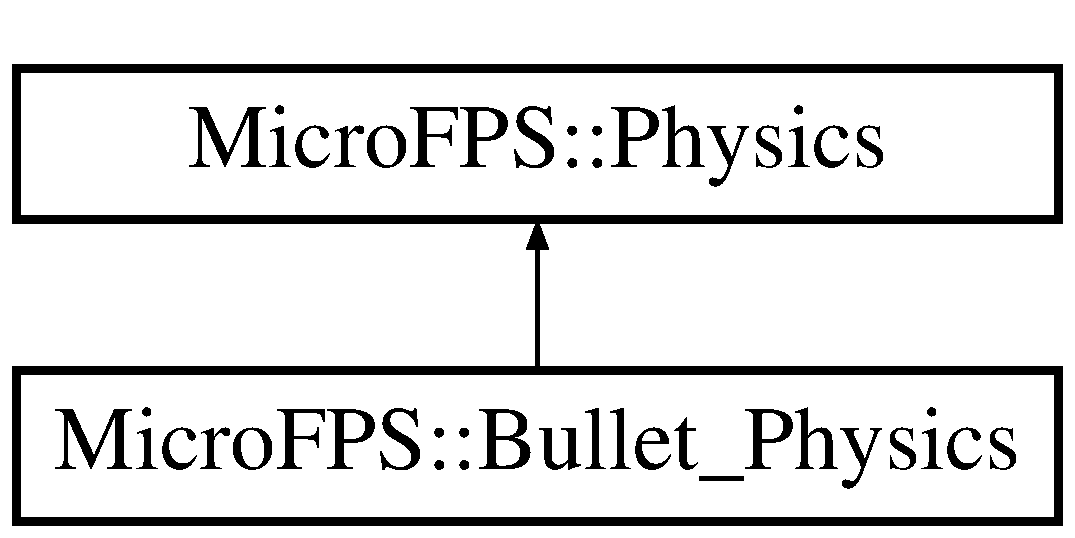
\includegraphics[height=2.000000cm]{da/d83/class_micro_f_p_s_1_1_bullet___physics}
\end{center}
\end{figure}
\subsection*{Public Member Functions}
\begin{DoxyCompactItemize}
\item 
\hyperlink{class_micro_f_p_s_1_1_bullet___physics_af563f8907ea77a2ed3d4f6f23d93aacc}{Bullet\_\-Physics} ()
\item 
virtual \hyperlink{class_micro_f_p_s_1_1_bullet___physics_a876f7933df0258d84c097b3996d86c72}{$\sim$Bullet\_\-Physics} ()
\item 
virtual physicsworld $\ast$ \hyperlink{class_micro_f_p_s_1_1_bullet___physics_aece8300cdd5ba7a0971cd3c30146d2af}{getWorld} () const 
\end{DoxyCompactItemize}


\subsection{Detailed Description}
\hyperlink{class_micro_f_p_s_1_1_bullet___physics}{Bullet\_\-Physics} Bullet physics connector 

\subsection{Constructor \& Destructor Documentation}
\hypertarget{class_micro_f_p_s_1_1_bullet___physics_af563f8907ea77a2ed3d4f6f23d93aacc}{
\index{MicroFPS::Bullet\_\-Physics@{MicroFPS::Bullet\_\-Physics}!Bullet\_\-Physics@{Bullet\_\-Physics}}
\index{Bullet\_\-Physics@{Bullet\_\-Physics}!MicroFPS::Bullet_Physics@{MicroFPS::Bullet\_\-Physics}}
\subsubsection[{Bullet\_\-Physics}]{\setlength{\rightskip}{0pt plus 5cm}MicroFPS::Bullet\_\-Physics::Bullet\_\-Physics (
\begin{DoxyParamCaption}
{}
\end{DoxyParamCaption}
)}}
\label{da/d83/class_micro_f_p_s_1_1_bullet___physics_af563f8907ea77a2ed3d4f6f23d93aacc}
Constructor \hypertarget{class_micro_f_p_s_1_1_bullet___physics_a876f7933df0258d84c097b3996d86c72}{
\index{MicroFPS::Bullet\_\-Physics@{MicroFPS::Bullet\_\-Physics}!$\sim$Bullet\_\-Physics@{$\sim$Bullet\_\-Physics}}
\index{$\sim$Bullet\_\-Physics@{$\sim$Bullet\_\-Physics}!MicroFPS::Bullet_Physics@{MicroFPS::Bullet\_\-Physics}}
\subsubsection[{$\sim$Bullet\_\-Physics}]{\setlength{\rightskip}{0pt plus 5cm}virtual MicroFPS::Bullet\_\-Physics::$\sim$Bullet\_\-Physics (
\begin{DoxyParamCaption}
{}
\end{DoxyParamCaption}
)\hspace{0.3cm}{\ttfamily  \mbox{[}virtual\mbox{]}}}}
\label{da/d83/class_micro_f_p_s_1_1_bullet___physics_a876f7933df0258d84c097b3996d86c72}
Destructor 

\subsection{Member Function Documentation}
\hypertarget{class_micro_f_p_s_1_1_bullet___physics_aece8300cdd5ba7a0971cd3c30146d2af}{
\index{MicroFPS::Bullet\_\-Physics@{MicroFPS::Bullet\_\-Physics}!getWorld@{getWorld}}
\index{getWorld@{getWorld}!MicroFPS::Bullet_Physics@{MicroFPS::Bullet\_\-Physics}}
\subsubsection[{getWorld}]{\setlength{\rightskip}{0pt plus 5cm}virtual physicsworld$\ast$ MicroFPS::Bullet\_\-Physics::getWorld (
\begin{DoxyParamCaption}
{}
\end{DoxyParamCaption}
) const\hspace{0.3cm}{\ttfamily  \mbox{[}virtual\mbox{]}}}}
\label{da/d83/class_micro_f_p_s_1_1_bullet___physics_aece8300cdd5ba7a0971cd3c30146d2af}
\hyperlink{class_micro_f_p_s_1_1_bullet___physics_aece8300cdd5ba7a0971cd3c30146d2af}{getWorld()} get the physics world 

Implements \hyperlink{class_micro_f_p_s_1_1_physics_a495b990b468be7a75c12f0e33df4f22c}{MicroFPS::Physics}.



The documentation for this class was generated from the following file:\begin{DoxyCompactItemize}
\item 
C:/Users/Dennis/Desktop/MicroFPS/src/MicroFPS/src/PhysicsEngines/Bullet\_\-Physics.h\end{DoxyCompactItemize}

\hypertarget{class_micro_f_p_s_1_1_game_manager}{
\section{MicroFPS::GameManager Class Reference}
\label{d8/d88/class_micro_f_p_s_1_1_game_manager}\index{MicroFPS::GameManager@{MicroFPS::GameManager}}
}


{\ttfamily \#include $<$GameManager.h$>$}

Inheritance diagram for MicroFPS::GameManager:\begin{figure}[H]
\begin{center}
\leavevmode
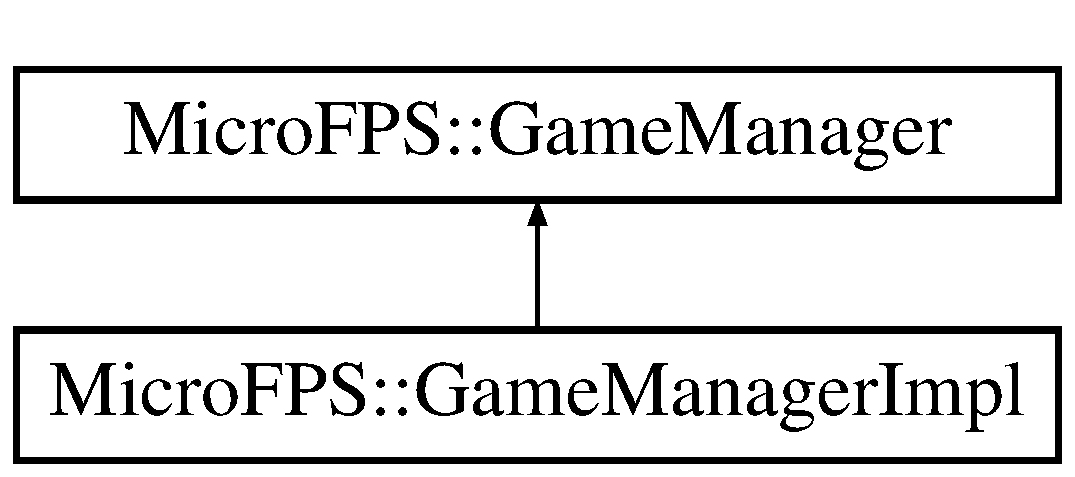
\includegraphics[height=2.000000cm]{d8/d88/class_micro_f_p_s_1_1_game_manager}
\end{center}
\end{figure}
\subsection*{Public Member Functions}
\begin{DoxyCompactItemize}
\item 
\hyperlink{class_micro_f_p_s_1_1_game_manager_ac51554cf7901660c82e9e706121e6711}{GameManager} ()
\item 
virtual \hyperlink{class_micro_f_p_s_1_1_game_manager_aade03d5fb5ef9c9474188fbb9a0a033a}{$\sim$GameManager} ()
\item 
virtual void \hyperlink{class_micro_f_p_s_1_1_game_manager_afce01403245a9266642fb609c3dd18de}{start} ()=0
\item 
virtual \hyperlink{class_micro_f_p_s_1_1_render_manager}{RenderManager} $\ast$ \hyperlink{class_micro_f_p_s_1_1_game_manager_ac8792976d8d44730864afb866f7ce7cc}{getRenderManager} () const =0
\item 
virtual \hyperlink{class_micro_f_p_s_1_1_state_manager}{StateManager} $\ast$ \hyperlink{class_micro_f_p_s_1_1_game_manager_ac8e2bed71b241e8e0463bdeb9175d844}{getStateManager} () const =0
\item 
virtual \hyperlink{class_micro_f_p_s_1_1_physics_manager}{PhysicsManager} $\ast$ \hyperlink{class_micro_f_p_s_1_1_game_manager_a5f7ba66d79351b6a3ce66c818ed73433}{getPhysicsManager} () const =0
\end{DoxyCompactItemize}


\subsection{Detailed Description}
\hyperlink{class_micro_f_p_s_1_1_game_manager}{GameManager} The glue to the entire system 

\subsection{Constructor \& Destructor Documentation}
\hypertarget{class_micro_f_p_s_1_1_game_manager_ac51554cf7901660c82e9e706121e6711}{
\index{MicroFPS::GameManager@{MicroFPS::GameManager}!GameManager@{GameManager}}
\index{GameManager@{GameManager}!MicroFPS::GameManager@{MicroFPS::GameManager}}
\subsubsection[{GameManager}]{\setlength{\rightskip}{0pt plus 5cm}MicroFPS::GameManager::GameManager (
\begin{DoxyParamCaption}
{}
\end{DoxyParamCaption}
)\hspace{0.3cm}{\ttfamily  \mbox{[}inline\mbox{]}}}}
\label{d8/d88/class_micro_f_p_s_1_1_game_manager_ac51554cf7901660c82e9e706121e6711}
\hyperlink{class_micro_f_p_s_1_1_game_manager_ac51554cf7901660c82e9e706121e6711}{GameManager()} General default constructor \hypertarget{class_micro_f_p_s_1_1_game_manager_aade03d5fb5ef9c9474188fbb9a0a033a}{
\index{MicroFPS::GameManager@{MicroFPS::GameManager}!$\sim$GameManager@{$\sim$GameManager}}
\index{$\sim$GameManager@{$\sim$GameManager}!MicroFPS::GameManager@{MicroFPS::GameManager}}
\subsubsection[{$\sim$GameManager}]{\setlength{\rightskip}{0pt plus 5cm}virtual MicroFPS::GameManager::$\sim$GameManager (
\begin{DoxyParamCaption}
{}
\end{DoxyParamCaption}
)\hspace{0.3cm}{\ttfamily  \mbox{[}inline, virtual\mbox{]}}}}
\label{d8/d88/class_micro_f_p_s_1_1_game_manager_aade03d5fb5ef9c9474188fbb9a0a033a}
\hyperlink{class_micro_f_p_s_1_1_game_manager_aade03d5fb5ef9c9474188fbb9a0a033a}{$\sim$GameManager()} Virtual destructor we're done 

\subsection{Member Function Documentation}
\hypertarget{class_micro_f_p_s_1_1_game_manager_a5f7ba66d79351b6a3ce66c818ed73433}{
\index{MicroFPS::GameManager@{MicroFPS::GameManager}!getPhysicsManager@{getPhysicsManager}}
\index{getPhysicsManager@{getPhysicsManager}!MicroFPS::GameManager@{MicroFPS::GameManager}}
\subsubsection[{getPhysicsManager}]{\setlength{\rightskip}{0pt plus 5cm}virtual {\bf PhysicsManager}$\ast$ MicroFPS::GameManager::getPhysicsManager (
\begin{DoxyParamCaption}
{}
\end{DoxyParamCaption}
) const\hspace{0.3cm}{\ttfamily  \mbox{[}pure virtual\mbox{]}}}}
\label{d8/d88/class_micro_f_p_s_1_1_game_manager_a5f7ba66d79351b6a3ce66c818ed73433}
getPhysicsManager Retrieve physics manager 

Implemented in \hyperlink{class_micro_f_p_s_1_1_game_manager_impl_af22a0a2d254220f1be1b0a92963d641e}{MicroFPS::GameManagerImpl}.

\hypertarget{class_micro_f_p_s_1_1_game_manager_ac8792976d8d44730864afb866f7ce7cc}{
\index{MicroFPS::GameManager@{MicroFPS::GameManager}!getRenderManager@{getRenderManager}}
\index{getRenderManager@{getRenderManager}!MicroFPS::GameManager@{MicroFPS::GameManager}}
\subsubsection[{getRenderManager}]{\setlength{\rightskip}{0pt plus 5cm}virtual {\bf RenderManager}$\ast$ MicroFPS::GameManager::getRenderManager (
\begin{DoxyParamCaption}
{}
\end{DoxyParamCaption}
) const\hspace{0.3cm}{\ttfamily  \mbox{[}pure virtual\mbox{]}}}}
\label{d8/d88/class_micro_f_p_s_1_1_game_manager_ac8792976d8d44730864afb866f7ce7cc}
\hyperlink{class_micro_f_p_s_1_1_game_manager_ac8792976d8d44730864afb866f7ce7cc}{getRenderManager()} Get the render manager 

Implemented in \hyperlink{class_micro_f_p_s_1_1_game_manager_impl_a8d6c455d801f35c335c6648ecc2adb66}{MicroFPS::GameManagerImpl}.

\hypertarget{class_micro_f_p_s_1_1_game_manager_ac8e2bed71b241e8e0463bdeb9175d844}{
\index{MicroFPS::GameManager@{MicroFPS::GameManager}!getStateManager@{getStateManager}}
\index{getStateManager@{getStateManager}!MicroFPS::GameManager@{MicroFPS::GameManager}}
\subsubsection[{getStateManager}]{\setlength{\rightskip}{0pt plus 5cm}virtual {\bf StateManager}$\ast$ MicroFPS::GameManager::getStateManager (
\begin{DoxyParamCaption}
{}
\end{DoxyParamCaption}
) const\hspace{0.3cm}{\ttfamily  \mbox{[}pure virtual\mbox{]}}}}
\label{d8/d88/class_micro_f_p_s_1_1_game_manager_ac8e2bed71b241e8e0463bdeb9175d844}
\hyperlink{class_micro_f_p_s_1_1_game_manager_ac8e2bed71b241e8e0463bdeb9175d844}{getStateManager()} Get the state manager 

Implemented in \hyperlink{class_micro_f_p_s_1_1_game_manager_impl_aeb67fb518616ef72d0f7b252d15908c4}{MicroFPS::GameManagerImpl}.

\hypertarget{class_micro_f_p_s_1_1_game_manager_afce01403245a9266642fb609c3dd18de}{
\index{MicroFPS::GameManager@{MicroFPS::GameManager}!start@{start}}
\index{start@{start}!MicroFPS::GameManager@{MicroFPS::GameManager}}
\subsubsection[{start}]{\setlength{\rightskip}{0pt plus 5cm}virtual void MicroFPS::GameManager::start (
\begin{DoxyParamCaption}
{}
\end{DoxyParamCaption}
)\hspace{0.3cm}{\ttfamily  \mbox{[}pure virtual\mbox{]}}}}
\label{d8/d88/class_micro_f_p_s_1_1_game_manager_afce01403245a9266642fb609c3dd18de}
start The function which will initialize the game loop 

Implemented in \hyperlink{class_micro_f_p_s_1_1_game_manager_impl_a408a6e2b5f22501b662cfd65c6437135}{MicroFPS::GameManagerImpl}.



The documentation for this class was generated from the following file:\begin{DoxyCompactItemize}
\item 
C:/Users/Dennis/Desktop/MicroFPS/src/MicroFPS/src/Managers/GameManager.h\end{DoxyCompactItemize}

\hypertarget{class_micro_f_p_s_1_1_game_manager_impl}{
\section{MicroFPS::GameManagerImpl Class Reference}
\label{d8/daa/class_micro_f_p_s_1_1_game_manager_impl}\index{MicroFPS::GameManagerImpl@{MicroFPS::GameManagerImpl}}
}


{\ttfamily \#include $<$GameManagerImpl.h$>$}

Inheritance diagram for MicroFPS::GameManagerImpl:\begin{figure}[H]
\begin{center}
\leavevmode
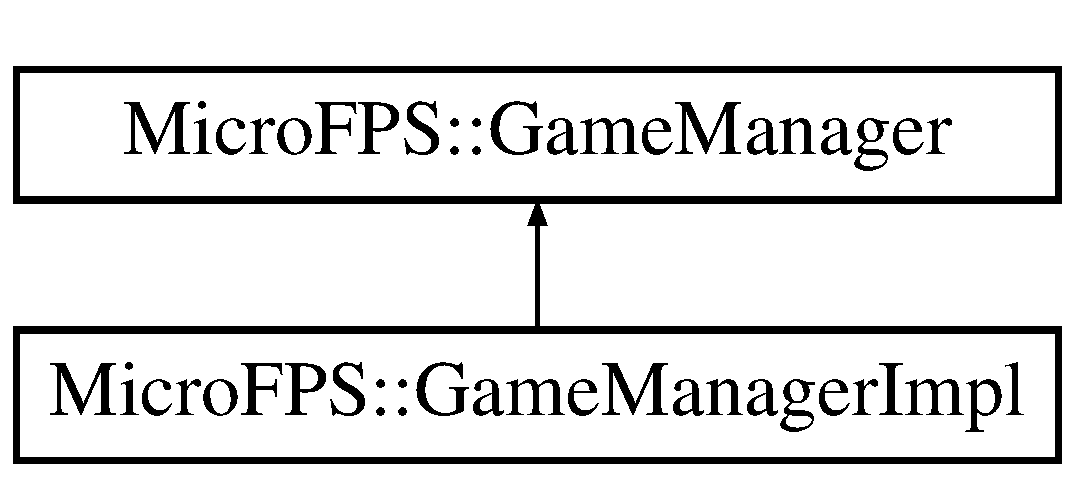
\includegraphics[height=2.000000cm]{d8/daa/class_micro_f_p_s_1_1_game_manager_impl}
\end{center}
\end{figure}
\subsection*{Public Member Functions}
\begin{DoxyCompactItemize}
\item 
\hyperlink{class_micro_f_p_s_1_1_game_manager_impl_a6408c200462f62b1ed86521b90c85b27}{GameManagerImpl} ()
\item 
virtual \hyperlink{class_micro_f_p_s_1_1_game_manager_impl_a8479ea0ec07612cefcadd46d10429866}{$\sim$GameManagerImpl} ()
\item 
virtual void \hyperlink{class_micro_f_p_s_1_1_game_manager_impl_a408a6e2b5f22501b662cfd65c6437135}{start} ()
\item 
virtual \hyperlink{class_micro_f_p_s_1_1_render_manager}{RenderManager} $\ast$ \hyperlink{class_micro_f_p_s_1_1_game_manager_impl_a8d6c455d801f35c335c6648ecc2adb66}{getRenderManager} () const 
\item 
virtual \hyperlink{class_micro_f_p_s_1_1_state_manager}{StateManager} $\ast$ \hyperlink{class_micro_f_p_s_1_1_game_manager_impl_aeb67fb518616ef72d0f7b252d15908c4}{getStateManager} () const 
\item 
virtual \hyperlink{class_micro_f_p_s_1_1_physics_manager}{PhysicsManager} $\ast$ \hyperlink{class_micro_f_p_s_1_1_game_manager_impl_af22a0a2d254220f1be1b0a92963d641e}{getPhysicsManager} () const 
\end{DoxyCompactItemize}


\subsection{Detailed Description}
\hyperlink{class_micro_f_p_s_1_1_game_manager_impl}{GameManagerImpl} Implementation of the Game Manager 

\subsection{Constructor \& Destructor Documentation}
\hypertarget{class_micro_f_p_s_1_1_game_manager_impl_a6408c200462f62b1ed86521b90c85b27}{
\index{MicroFPS::GameManagerImpl@{MicroFPS::GameManagerImpl}!GameManagerImpl@{GameManagerImpl}}
\index{GameManagerImpl@{GameManagerImpl}!MicroFPS::GameManagerImpl@{MicroFPS::GameManagerImpl}}
\subsubsection[{GameManagerImpl}]{\setlength{\rightskip}{0pt plus 5cm}MicroFPS::GameManagerImpl::GameManagerImpl (
\begin{DoxyParamCaption}
{}
\end{DoxyParamCaption}
)}}
\label{d8/daa/class_micro_f_p_s_1_1_game_manager_impl_a6408c200462f62b1ed86521b90c85b27}
\hyperlink{class_micro_f_p_s_1_1_game_manager_impl_a6408c200462f62b1ed86521b90c85b27}{GameManagerImpl()} General Constructor \hypertarget{class_micro_f_p_s_1_1_game_manager_impl_a8479ea0ec07612cefcadd46d10429866}{
\index{MicroFPS::GameManagerImpl@{MicroFPS::GameManagerImpl}!$\sim$GameManagerImpl@{$\sim$GameManagerImpl}}
\index{$\sim$GameManagerImpl@{$\sim$GameManagerImpl}!MicroFPS::GameManagerImpl@{MicroFPS::GameManagerImpl}}
\subsubsection[{$\sim$GameManagerImpl}]{\setlength{\rightskip}{0pt plus 5cm}virtual MicroFPS::GameManagerImpl::$\sim$GameManagerImpl (
\begin{DoxyParamCaption}
{}
\end{DoxyParamCaption}
)\hspace{0.3cm}{\ttfamily  \mbox{[}virtual\mbox{]}}}}
\label{d8/daa/class_micro_f_p_s_1_1_game_manager_impl_a8479ea0ec07612cefcadd46d10429866}
\hyperlink{class_micro_f_p_s_1_1_game_manager_impl_a8479ea0ec07612cefcadd46d10429866}{$\sim$GameManagerImpl()} Standard virtual destructor 

\subsection{Member Function Documentation}
\hypertarget{class_micro_f_p_s_1_1_game_manager_impl_af22a0a2d254220f1be1b0a92963d641e}{
\index{MicroFPS::GameManagerImpl@{MicroFPS::GameManagerImpl}!getPhysicsManager@{getPhysicsManager}}
\index{getPhysicsManager@{getPhysicsManager}!MicroFPS::GameManagerImpl@{MicroFPS::GameManagerImpl}}
\subsubsection[{getPhysicsManager}]{\setlength{\rightskip}{0pt plus 5cm}virtual {\bf PhysicsManager}$\ast$ MicroFPS::GameManagerImpl::getPhysicsManager (
\begin{DoxyParamCaption}
{}
\end{DoxyParamCaption}
) const\hspace{0.3cm}{\ttfamily  \mbox{[}virtual\mbox{]}}}}
\label{d8/daa/class_micro_f_p_s_1_1_game_manager_impl_af22a0a2d254220f1be1b0a92963d641e}
getPhysicsManager Retrieve physics manager 

Implements \hyperlink{class_micro_f_p_s_1_1_game_manager_a5f7ba66d79351b6a3ce66c818ed73433}{MicroFPS::GameManager}.

\hypertarget{class_micro_f_p_s_1_1_game_manager_impl_a8d6c455d801f35c335c6648ecc2adb66}{
\index{MicroFPS::GameManagerImpl@{MicroFPS::GameManagerImpl}!getRenderManager@{getRenderManager}}
\index{getRenderManager@{getRenderManager}!MicroFPS::GameManagerImpl@{MicroFPS::GameManagerImpl}}
\subsubsection[{getRenderManager}]{\setlength{\rightskip}{0pt plus 5cm}virtual {\bf RenderManager}$\ast$ MicroFPS::GameManagerImpl::getRenderManager (
\begin{DoxyParamCaption}
{}
\end{DoxyParamCaption}
) const\hspace{0.3cm}{\ttfamily  \mbox{[}virtual\mbox{]}}}}
\label{d8/daa/class_micro_f_p_s_1_1_game_manager_impl_a8d6c455d801f35c335c6648ecc2adb66}
\hyperlink{class_micro_f_p_s_1_1_game_manager_impl_a8d6c455d801f35c335c6648ecc2adb66}{getRenderManager()} Get the render manager 

Implements \hyperlink{class_micro_f_p_s_1_1_game_manager_ac8792976d8d44730864afb866f7ce7cc}{MicroFPS::GameManager}.

\hypertarget{class_micro_f_p_s_1_1_game_manager_impl_aeb67fb518616ef72d0f7b252d15908c4}{
\index{MicroFPS::GameManagerImpl@{MicroFPS::GameManagerImpl}!getStateManager@{getStateManager}}
\index{getStateManager@{getStateManager}!MicroFPS::GameManagerImpl@{MicroFPS::GameManagerImpl}}
\subsubsection[{getStateManager}]{\setlength{\rightskip}{0pt plus 5cm}virtual {\bf StateManager}$\ast$ MicroFPS::GameManagerImpl::getStateManager (
\begin{DoxyParamCaption}
{}
\end{DoxyParamCaption}
) const\hspace{0.3cm}{\ttfamily  \mbox{[}virtual\mbox{]}}}}
\label{d8/daa/class_micro_f_p_s_1_1_game_manager_impl_aeb67fb518616ef72d0f7b252d15908c4}
getStateManager Retrieve the state manager 

Implements \hyperlink{class_micro_f_p_s_1_1_game_manager_ac8e2bed71b241e8e0463bdeb9175d844}{MicroFPS::GameManager}.

\hypertarget{class_micro_f_p_s_1_1_game_manager_impl_a408a6e2b5f22501b662cfd65c6437135}{
\index{MicroFPS::GameManagerImpl@{MicroFPS::GameManagerImpl}!start@{start}}
\index{start@{start}!MicroFPS::GameManagerImpl@{MicroFPS::GameManagerImpl}}
\subsubsection[{start}]{\setlength{\rightskip}{0pt plus 5cm}virtual void MicroFPS::GameManagerImpl::start (
\begin{DoxyParamCaption}
{}
\end{DoxyParamCaption}
)\hspace{0.3cm}{\ttfamily  \mbox{[}virtual\mbox{]}}}}
\label{d8/daa/class_micro_f_p_s_1_1_game_manager_impl_a408a6e2b5f22501b662cfd65c6437135}
\hyperlink{class_micro_f_p_s_1_1_game_manager_impl_a408a6e2b5f22501b662cfd65c6437135}{start()} Initializes the game loop \begin{DoxyReturn}{Returns}
void 
\end{DoxyReturn}


Implements \hyperlink{class_micro_f_p_s_1_1_game_manager_afce01403245a9266642fb609c3dd18de}{MicroFPS::GameManager}.



The documentation for this class was generated from the following file:\begin{DoxyCompactItemize}
\item 
C:/Users/Dennis/Desktop/MicroFPS/src/MicroFPS/src/Managers/GameManagerImpl.h\end{DoxyCompactItemize}

\hypertarget{class_micro_f_p_s_1_1_game_state}{
\section{MicroFPS::GameState Class Reference}
\label{df/dc6/class_micro_f_p_s_1_1_game_state}\index{MicroFPS::GameState@{MicroFPS::GameState}}
}


{\ttfamily \#include $<$GameState.h$>$}

Inheritance diagram for MicroFPS::GameState:\begin{figure}[H]
\begin{center}
\leavevmode
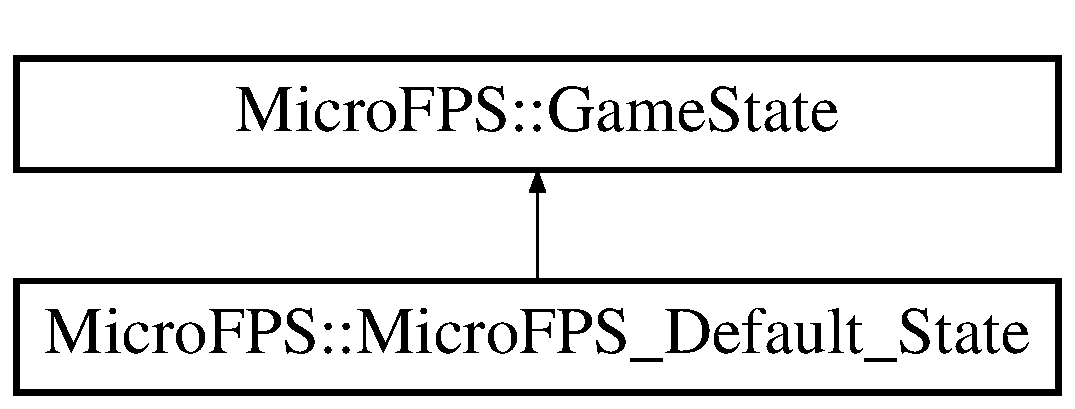
\includegraphics[height=2.000000cm]{df/dc6/class_micro_f_p_s_1_1_game_state}
\end{center}
\end{figure}
\subsection*{Public Types}
\begin{DoxyCompactItemize}
\item 
enum \hyperlink{class_micro_f_p_s_1_1_game_state_a2473115955f3009dae963b45f6a45ef3}{STATE\_\-TYPE} \{ {\bfseries LEVEL}, 
{\bfseries MENU}
 \}
\end{DoxyCompactItemize}
\subsection*{Public Member Functions}
\begin{DoxyCompactItemize}
\item 
\hyperlink{class_micro_f_p_s_1_1_game_state_a9ff190c74054ce2a3f5f5dd82601fc42}{GameState} ()
\item 
virtual \hyperlink{class_micro_f_p_s_1_1_game_state_ac7ed58f354a2a1e5d1942f5d361a9dab}{$\sim$GameState} ()
\item 
virtual void \hyperlink{class_micro_f_p_s_1_1_game_state_ac14111702f8eb2bae5f24102f585be92}{criticalLoop} ()=0
\item 
virtual void \hyperlink{class_micro_f_p_s_1_1_game_state_abb50cf29131b2099d78021de1322d778}{gameLoop} ()=0
\item 
virtual void \hyperlink{class_micro_f_p_s_1_1_game_state_a45db2d9ce96ac103465f798145f86927}{change} ()=0
\item 
virtual void \hyperlink{class_micro_f_p_s_1_1_game_state_a3e8da39e3c244a903a4e26252f9856a6}{leave} ()=0
\item 
virtual scenemgr \hyperlink{class_micro_f_p_s_1_1_game_state_a0b4c12fd50d7250e08ae82594231b0ef}{getSceneManager} () const =0
\item 
virtual GUI $\ast$ \hyperlink{class_micro_f_p_s_1_1_game_state_aa56075c68fd9dddc15cf067c5626e507}{getGUI} () const =0
\end{DoxyCompactItemize}


\subsection{Detailed Description}
\hyperlink{class_micro_f_p_s_1_1_game_state}{GameState} Determine what a \hyperlink{class_micro_f_p_s_1_1_game_state}{GameState} consists of 

\subsection{Member Enumeration Documentation}
\hypertarget{class_micro_f_p_s_1_1_game_state_a2473115955f3009dae963b45f6a45ef3}{
\index{MicroFPS::GameState@{MicroFPS::GameState}!STATE\_\-TYPE@{STATE\_\-TYPE}}
\index{STATE\_\-TYPE@{STATE\_\-TYPE}!MicroFPS::GameState@{MicroFPS::GameState}}
\subsubsection[{STATE\_\-TYPE}]{\setlength{\rightskip}{0pt plus 5cm}enum {\bf MicroFPS::GameState::STATE\_\-TYPE}}}
\label{df/dc6/class_micro_f_p_s_1_1_game_state_a2473115955f3009dae963b45f6a45ef3}
STATE\_\-TYPE ENUM to determine type of state 

\subsection{Constructor \& Destructor Documentation}
\hypertarget{class_micro_f_p_s_1_1_game_state_a9ff190c74054ce2a3f5f5dd82601fc42}{
\index{MicroFPS::GameState@{MicroFPS::GameState}!GameState@{GameState}}
\index{GameState@{GameState}!MicroFPS::GameState@{MicroFPS::GameState}}
\subsubsection[{GameState}]{\setlength{\rightskip}{0pt plus 5cm}MicroFPS::GameState::GameState (
\begin{DoxyParamCaption}
{}
\end{DoxyParamCaption}
)\hspace{0.3cm}{\ttfamily  \mbox{[}inline\mbox{]}}}}
\label{df/dc6/class_micro_f_p_s_1_1_game_state_a9ff190c74054ce2a3f5f5dd82601fc42}
Constructor \hypertarget{class_micro_f_p_s_1_1_game_state_ac7ed58f354a2a1e5d1942f5d361a9dab}{
\index{MicroFPS::GameState@{MicroFPS::GameState}!$\sim$GameState@{$\sim$GameState}}
\index{$\sim$GameState@{$\sim$GameState}!MicroFPS::GameState@{MicroFPS::GameState}}
\subsubsection[{$\sim$GameState}]{\setlength{\rightskip}{0pt plus 5cm}virtual MicroFPS::GameState::$\sim$GameState (
\begin{DoxyParamCaption}
{}
\end{DoxyParamCaption}
)\hspace{0.3cm}{\ttfamily  \mbox{[}inline, virtual\mbox{]}}}}
\label{df/dc6/class_micro_f_p_s_1_1_game_state_ac7ed58f354a2a1e5d1942f5d361a9dab}
Destructor 

\subsection{Member Function Documentation}
\hypertarget{class_micro_f_p_s_1_1_game_state_a45db2d9ce96ac103465f798145f86927}{
\index{MicroFPS::GameState@{MicroFPS::GameState}!change@{change}}
\index{change@{change}!MicroFPS::GameState@{MicroFPS::GameState}}
\subsubsection[{change}]{\setlength{\rightskip}{0pt plus 5cm}virtual void MicroFPS::GameState::change (
\begin{DoxyParamCaption}
{}
\end{DoxyParamCaption}
)\hspace{0.3cm}{\ttfamily  \mbox{[}pure virtual\mbox{]}}}}
\label{df/dc6/class_micro_f_p_s_1_1_game_state_a45db2d9ce96ac103465f798145f86927}
\hyperlink{class_micro_f_p_s_1_1_game_state_a45db2d9ce96ac103465f798145f86927}{change()} Void function to simply prepare the state to be viewed 

Implemented in \hyperlink{class_micro_f_p_s_1_1_micro_f_p_s___default___state_a991dd2a5c3447ffbfc2a3273ecee3dde}{MicroFPS::MicroFPS\_\-Default\_\-State}.

\hypertarget{class_micro_f_p_s_1_1_game_state_ac14111702f8eb2bae5f24102f585be92}{
\index{MicroFPS::GameState@{MicroFPS::GameState}!criticalLoop@{criticalLoop}}
\index{criticalLoop@{criticalLoop}!MicroFPS::GameState@{MicroFPS::GameState}}
\subsubsection[{criticalLoop}]{\setlength{\rightskip}{0pt plus 5cm}virtual void MicroFPS::GameState::criticalLoop (
\begin{DoxyParamCaption}
{}
\end{DoxyParamCaption}
)\hspace{0.3cm}{\ttfamily  \mbox{[}pure virtual\mbox{]}}}}
\label{df/dc6/class_micro_f_p_s_1_1_game_state_ac14111702f8eb2bae5f24102f585be92}
criticalLoop Determine what to add (if anything) to the predefined game loop (this happens during rendering)
\begin{DoxyItemize}
\item time critical stuff (don't put things here unless they need to be) 
\end{DoxyItemize}

Implemented in \hyperlink{class_micro_f_p_s_1_1_micro_f_p_s___default___state_ad1244341dd3c899b326eae64d9cf62a5}{MicroFPS::MicroFPS\_\-Default\_\-State}.

\hypertarget{class_micro_f_p_s_1_1_game_state_abb50cf29131b2099d78021de1322d778}{
\index{MicroFPS::GameState@{MicroFPS::GameState}!gameLoop@{gameLoop}}
\index{gameLoop@{gameLoop}!MicroFPS::GameState@{MicroFPS::GameState}}
\subsubsection[{gameLoop}]{\setlength{\rightskip}{0pt plus 5cm}virtual void MicroFPS::GameState::gameLoop (
\begin{DoxyParamCaption}
{}
\end{DoxyParamCaption}
)\hspace{0.3cm}{\ttfamily  \mbox{[}pure virtual\mbox{]}}}}
\label{df/dc6/class_micro_f_p_s_1_1_game_state_abb50cf29131b2099d78021de1322d778}
gameLoop The normal game loop (post scene render) 

Implemented in \hyperlink{class_micro_f_p_s_1_1_micro_f_p_s___default___state_a5e1c596521adde8a507837984a91ea52}{MicroFPS::MicroFPS\_\-Default\_\-State}.

\hypertarget{class_micro_f_p_s_1_1_game_state_aa56075c68fd9dddc15cf067c5626e507}{
\index{MicroFPS::GameState@{MicroFPS::GameState}!getGUI@{getGUI}}
\index{getGUI@{getGUI}!MicroFPS::GameState@{MicroFPS::GameState}}
\subsubsection[{getGUI}]{\setlength{\rightskip}{0pt plus 5cm}virtual GUI$\ast$ MicroFPS::GameState::getGUI (
\begin{DoxyParamCaption}
{}
\end{DoxyParamCaption}
) const\hspace{0.3cm}{\ttfamily  \mbox{[}pure virtual\mbox{]}}}}
\label{df/dc6/class_micro_f_p_s_1_1_game_state_aa56075c68fd9dddc15cf067c5626e507}
getGUI get GUI object 

Implemented in \hyperlink{class_micro_f_p_s_1_1_micro_f_p_s___default___state_acfac42fbdd87539dd9bf16a100304825}{MicroFPS::MicroFPS\_\-Default\_\-State}.

\hypertarget{class_micro_f_p_s_1_1_game_state_a0b4c12fd50d7250e08ae82594231b0ef}{
\index{MicroFPS::GameState@{MicroFPS::GameState}!getSceneManager@{getSceneManager}}
\index{getSceneManager@{getSceneManager}!MicroFPS::GameState@{MicroFPS::GameState}}
\subsubsection[{getSceneManager}]{\setlength{\rightskip}{0pt plus 5cm}virtual scenemgr MicroFPS::GameState::getSceneManager (
\begin{DoxyParamCaption}
{}
\end{DoxyParamCaption}
) const\hspace{0.3cm}{\ttfamily  \mbox{[}pure virtual\mbox{]}}}}
\label{df/dc6/class_micro_f_p_s_1_1_game_state_a0b4c12fd50d7250e08ae82594231b0ef}
getSceneManager get the scene manager for the state 

Implemented in \hyperlink{class_micro_f_p_s_1_1_micro_f_p_s___default___state_abca8b7a177d52cdc1b722afb34e393e4}{MicroFPS::MicroFPS\_\-Default\_\-State}.

\hypertarget{class_micro_f_p_s_1_1_game_state_a3e8da39e3c244a903a4e26252f9856a6}{
\index{MicroFPS::GameState@{MicroFPS::GameState}!leave@{leave}}
\index{leave@{leave}!MicroFPS::GameState@{MicroFPS::GameState}}
\subsubsection[{leave}]{\setlength{\rightskip}{0pt plus 5cm}virtual void MicroFPS::GameState::leave (
\begin{DoxyParamCaption}
{}
\end{DoxyParamCaption}
)\hspace{0.3cm}{\ttfamily  \mbox{[}pure virtual\mbox{]}}}}
\label{df/dc6/class_micro_f_p_s_1_1_game_state_a3e8da39e3c244a903a4e26252f9856a6}
\hyperlink{class_micro_f_p_s_1_1_game_state_a3e8da39e3c244a903a4e26252f9856a6}{leave()} Prepare a scene to be left 

Implemented in \hyperlink{class_micro_f_p_s_1_1_micro_f_p_s___default___state_a153a9771384034079df9419872d0b730}{MicroFPS::MicroFPS\_\-Default\_\-State}.



The documentation for this class was generated from the following file:\begin{DoxyCompactItemize}
\item 
C:/Users/Dennis/Desktop/MicroFPS/src/MicroFPS/src/States/GameState.h\end{DoxyCompactItemize}

\hypertarget{class_micro_f_p_s_1_1_irrlicht___renderer}{
\section{MicroFPS::Irrlicht\_\-Renderer Class Reference}
\label{d5/d5b/class_micro_f_p_s_1_1_irrlicht___renderer}\index{MicroFPS::Irrlicht\_\-Renderer@{MicroFPS::Irrlicht\_\-Renderer}}
}


{\ttfamily \#include $<$Irrlicht\_\-Renderer.h$>$}

Inheritance diagram for MicroFPS::Irrlicht\_\-Renderer:\begin{figure}[H]
\begin{center}
\leavevmode
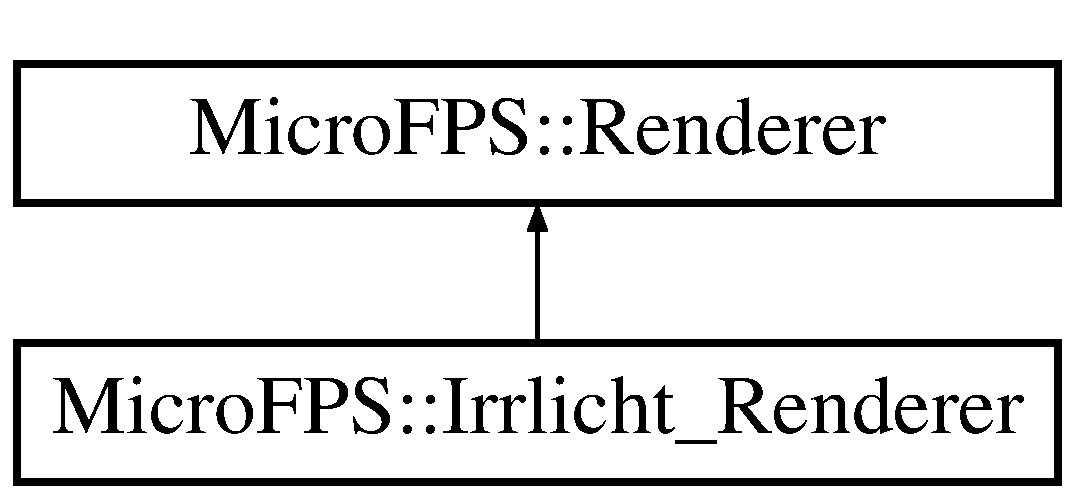
\includegraphics[height=2.000000cm]{d5/d5b/class_micro_f_p_s_1_1_irrlicht___renderer}
\end{center}
\end{figure}
\subsection*{Public Member Functions}
\begin{DoxyCompactItemize}
\item 
\hyperlink{class_micro_f_p_s_1_1_irrlicht___renderer_a9310435cb940f83daa7ec4e1b05ae555}{Irrlicht\_\-Renderer} (irr::video::E\_\-DRIVER\_\-TYPE driver=irr::video::EDT\_\-OPENGL, const irr::core::dimension2d$<$ irr::u32 $>$ \&windowSize=irr::core::dimension2d$<$ irr::u32 $>$(800, 600), irr::u32 bits=16, bool fullscreen=false, bool stencilbuffer=false, bool vsync=false)
\item 
virtual \hyperlink{class_micro_f_p_s_1_1_irrlicht___renderer_ab558709a3d5c1e582b00cb16bc3a5205}{$\sim$Irrlicht\_\-Renderer} ()
\item 
virtual renderer \hyperlink{class_micro_f_p_s_1_1_irrlicht___renderer_a6150c60d9599047f2d0ce468d4b3ac56}{getRendererDevice} () const 
\item 
virtual void \hyperlink{class_micro_f_p_s_1_1_irrlicht___renderer_ac719b88be714f1ece203d6dc3cce7ae2}{gameLoop} ()
\end{DoxyCompactItemize}


\subsection{Detailed Description}
\hyperlink{class_micro_f_p_s_1_1_irrlicht___renderer}{Irrlicht\_\-Renderer} Irrlicht renderer connector 

\subsection{Constructor \& Destructor Documentation}
\hypertarget{class_micro_f_p_s_1_1_irrlicht___renderer_a9310435cb940f83daa7ec4e1b05ae555}{
\index{MicroFPS::Irrlicht\_\-Renderer@{MicroFPS::Irrlicht\_\-Renderer}!Irrlicht\_\-Renderer@{Irrlicht\_\-Renderer}}
\index{Irrlicht\_\-Renderer@{Irrlicht\_\-Renderer}!MicroFPS::Irrlicht_Renderer@{MicroFPS::Irrlicht\_\-Renderer}}
\subsubsection[{Irrlicht\_\-Renderer}]{\setlength{\rightskip}{0pt plus 5cm}MicroFPS::Irrlicht\_\-Renderer::Irrlicht\_\-Renderer (
\begin{DoxyParamCaption}
\item[{irr::video::E\_\-DRIVER\_\-TYPE}]{driver = {\ttfamily irr::video::EDT\_\-OPENGL}, }
\item[{const irr::core::dimension2d$<$ irr::u32 $>$ \&}]{windowSize = {\ttfamily irr::core::dimension2d$<$~irr::u32~$>$(800,~600)}, }
\item[{irr::u32}]{bits = {\ttfamily 16}, }
\item[{bool}]{fullscreen = {\ttfamily false}, }
\item[{bool}]{stencilbuffer = {\ttfamily false}, }
\item[{bool}]{vsync = {\ttfamily false}}
\end{DoxyParamCaption}
)}}
\label{d5/d5b/class_micro_f_p_s_1_1_irrlicht___renderer_a9310435cb940f83daa7ec4e1b05ae555}
Constructor 
\begin{DoxyParams}{Parameters}
{\em irr::video::E\_\-DRIVER\_\-TYPE} & driver -\/ driver type \\
\hline
{\em irr::core::dimension2d$<$u32$>$} & windowSize -\/ window dimensions \\
\hline
{\em irr::u32} & bits -\/ display bits \\
\hline
{\em bool} & fullscreen -\/ Fullscreen mode? \\
\hline
{\em bool} & stencilbuffer -\/ Enable stencil buffer? \\
\hline
{\em bool} & vsync -\/ Enable vsync? \\
\hline
\end{DoxyParams}
\hypertarget{class_micro_f_p_s_1_1_irrlicht___renderer_ab558709a3d5c1e582b00cb16bc3a5205}{
\index{MicroFPS::Irrlicht\_\-Renderer@{MicroFPS::Irrlicht\_\-Renderer}!$\sim$Irrlicht\_\-Renderer@{$\sim$Irrlicht\_\-Renderer}}
\index{$\sim$Irrlicht\_\-Renderer@{$\sim$Irrlicht\_\-Renderer}!MicroFPS::Irrlicht_Renderer@{MicroFPS::Irrlicht\_\-Renderer}}
\subsubsection[{$\sim$Irrlicht\_\-Renderer}]{\setlength{\rightskip}{0pt plus 5cm}virtual MicroFPS::Irrlicht\_\-Renderer::$\sim$Irrlicht\_\-Renderer (
\begin{DoxyParamCaption}
{}
\end{DoxyParamCaption}
)\hspace{0.3cm}{\ttfamily  \mbox{[}virtual\mbox{]}}}}
\label{d5/d5b/class_micro_f_p_s_1_1_irrlicht___renderer_ab558709a3d5c1e582b00cb16bc3a5205}
Destructor 

\subsection{Member Function Documentation}
\hypertarget{class_micro_f_p_s_1_1_irrlicht___renderer_ac719b88be714f1ece203d6dc3cce7ae2}{
\index{MicroFPS::Irrlicht\_\-Renderer@{MicroFPS::Irrlicht\_\-Renderer}!gameLoop@{gameLoop}}
\index{gameLoop@{gameLoop}!MicroFPS::Irrlicht_Renderer@{MicroFPS::Irrlicht\_\-Renderer}}
\subsubsection[{gameLoop}]{\setlength{\rightskip}{0pt plus 5cm}virtual void MicroFPS::Irrlicht\_\-Renderer::gameLoop (
\begin{DoxyParamCaption}
{}
\end{DoxyParamCaption}
)\hspace{0.3cm}{\ttfamily  \mbox{[}virtual\mbox{]}}}}
\label{d5/d5b/class_micro_f_p_s_1_1_irrlicht___renderer_ac719b88be714f1ece203d6dc3cce7ae2}
gameLoop 

Implements \hyperlink{class_micro_f_p_s_1_1_renderer_a855df0a5be7f49d50f5de6be106376c3}{MicroFPS::Renderer}.

\hypertarget{class_micro_f_p_s_1_1_irrlicht___renderer_a6150c60d9599047f2d0ce468d4b3ac56}{
\index{MicroFPS::Irrlicht\_\-Renderer@{MicroFPS::Irrlicht\_\-Renderer}!getRendererDevice@{getRendererDevice}}
\index{getRendererDevice@{getRendererDevice}!MicroFPS::Irrlicht_Renderer@{MicroFPS::Irrlicht\_\-Renderer}}
\subsubsection[{getRendererDevice}]{\setlength{\rightskip}{0pt plus 5cm}virtual renderer MicroFPS::Irrlicht\_\-Renderer::getRendererDevice (
\begin{DoxyParamCaption}
{}
\end{DoxyParamCaption}
) const\hspace{0.3cm}{\ttfamily  \mbox{[}virtual\mbox{]}}}}
\label{d5/d5b/class_micro_f_p_s_1_1_irrlicht___renderer_a6150c60d9599047f2d0ce468d4b3ac56}
getRendererDevice get an irr::IrrlichtDevice 

Implements \hyperlink{class_micro_f_p_s_1_1_renderer_a092a7585391cd2a6067c80d8d989e8dd}{MicroFPS::Renderer}.



The documentation for this class was generated from the following file:\begin{DoxyCompactItemize}
\item 
C:/Users/Dennis/Desktop/MicroFPS/src/MicroFPS/src/RenderEngines/Irrlicht\_\-Renderer.h\end{DoxyCompactItemize}

\hypertarget{class_micro_f_p_s_1_1_physics}{
\section{MicroFPS::Physics Class Reference}
\label{d1/d3c/class_micro_f_p_s_1_1_physics}\index{MicroFPS::Physics@{MicroFPS::Physics}}
}


{\ttfamily \#include $<$Physics.h$>$}

Inheritance diagram for MicroFPS::Physics:\begin{figure}[H]
\begin{center}
\leavevmode
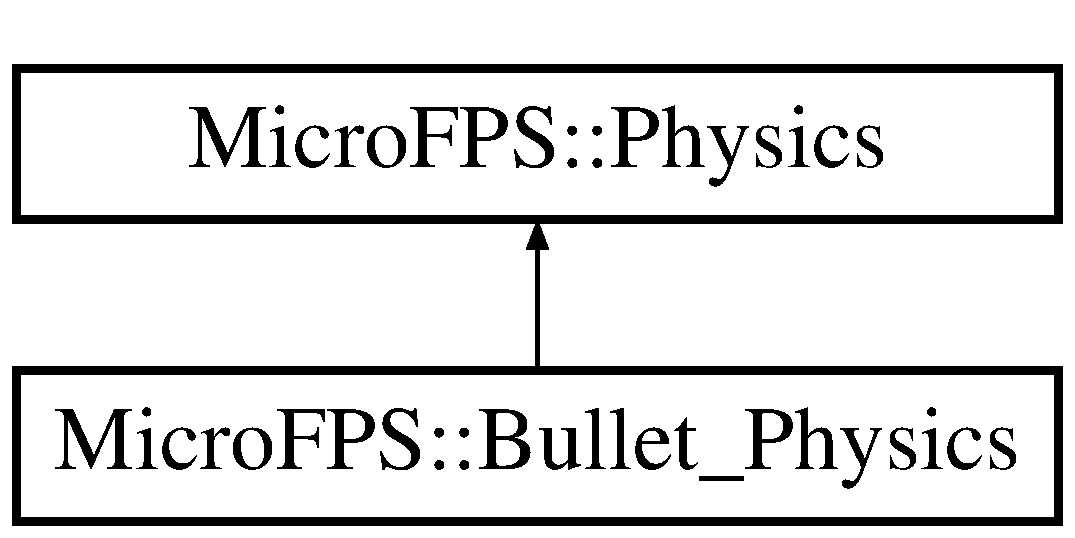
\includegraphics[height=2.000000cm]{d1/d3c/class_micro_f_p_s_1_1_physics}
\end{center}
\end{figure}
\subsection*{Public Member Functions}
\begin{DoxyCompactItemize}
\item 
\hyperlink{class_micro_f_p_s_1_1_physics_a3bf3fa711f8928147492455497a585d3}{Physics} ()
\item 
virtual \hyperlink{class_micro_f_p_s_1_1_physics_a82f717fa1826fe7c0a9187c33ec2c994}{$\sim$Physics} ()
\item 
virtual physicsworld $\ast$ \hyperlink{class_micro_f_p_s_1_1_physics_a495b990b468be7a75c12f0e33df4f22c}{getWorld} () const =0
\end{DoxyCompactItemize}


\subsection{Detailed Description}
\hyperlink{class_micro_f_p_s_1_1_physics}{Physics} \hyperlink{class_micro_f_p_s_1_1_physics}{Physics} abstract base class 

\subsection{Constructor \& Destructor Documentation}
\hypertarget{class_micro_f_p_s_1_1_physics_a3bf3fa711f8928147492455497a585d3}{
\index{MicroFPS::Physics@{MicroFPS::Physics}!Physics@{Physics}}
\index{Physics@{Physics}!MicroFPS::Physics@{MicroFPS::Physics}}
\subsubsection[{Physics}]{\setlength{\rightskip}{0pt plus 5cm}MicroFPS::Physics::Physics (
\begin{DoxyParamCaption}
{}
\end{DoxyParamCaption}
)\hspace{0.3cm}{\ttfamily  \mbox{[}inline\mbox{]}}}}
\label{d1/d3c/class_micro_f_p_s_1_1_physics_a3bf3fa711f8928147492455497a585d3}
Constructor \hypertarget{class_micro_f_p_s_1_1_physics_a82f717fa1826fe7c0a9187c33ec2c994}{
\index{MicroFPS::Physics@{MicroFPS::Physics}!$\sim$Physics@{$\sim$Physics}}
\index{$\sim$Physics@{$\sim$Physics}!MicroFPS::Physics@{MicroFPS::Physics}}
\subsubsection[{$\sim$Physics}]{\setlength{\rightskip}{0pt plus 5cm}virtual MicroFPS::Physics::$\sim$Physics (
\begin{DoxyParamCaption}
{}
\end{DoxyParamCaption}
)\hspace{0.3cm}{\ttfamily  \mbox{[}inline, virtual\mbox{]}}}}
\label{d1/d3c/class_micro_f_p_s_1_1_physics_a82f717fa1826fe7c0a9187c33ec2c994}
Destructor 

\subsection{Member Function Documentation}
\hypertarget{class_micro_f_p_s_1_1_physics_a495b990b468be7a75c12f0e33df4f22c}{
\index{MicroFPS::Physics@{MicroFPS::Physics}!getWorld@{getWorld}}
\index{getWorld@{getWorld}!MicroFPS::Physics@{MicroFPS::Physics}}
\subsubsection[{getWorld}]{\setlength{\rightskip}{0pt plus 5cm}virtual physicsworld$\ast$ MicroFPS::Physics::getWorld (
\begin{DoxyParamCaption}
{}
\end{DoxyParamCaption}
) const\hspace{0.3cm}{\ttfamily  \mbox{[}pure virtual\mbox{]}}}}
\label{d1/d3c/class_micro_f_p_s_1_1_physics_a495b990b468be7a75c12f0e33df4f22c}
getWorld 

Implemented in \hyperlink{class_micro_f_p_s_1_1_bullet___physics_aece8300cdd5ba7a0971cd3c30146d2af}{MicroFPS::Bullet\_\-Physics}.



The documentation for this class was generated from the following file:\begin{DoxyCompactItemize}
\item 
C:/Users/Dennis/Desktop/MicroFPS/src/MicroFPS/src/PhysicsEngines/Physics.h\end{DoxyCompactItemize}

\hypertarget{class_micro_f_p_s_1_1_physics_manager}{
\section{MicroFPS::PhysicsManager Class Reference}
\label{db/d08/class_micro_f_p_s_1_1_physics_manager}\index{MicroFPS::PhysicsManager@{MicroFPS::PhysicsManager}}
}


{\ttfamily \#include $<$PhysicsManager.h$>$}

Inheritance diagram for MicroFPS::PhysicsManager:\begin{figure}[H]
\begin{center}
\leavevmode
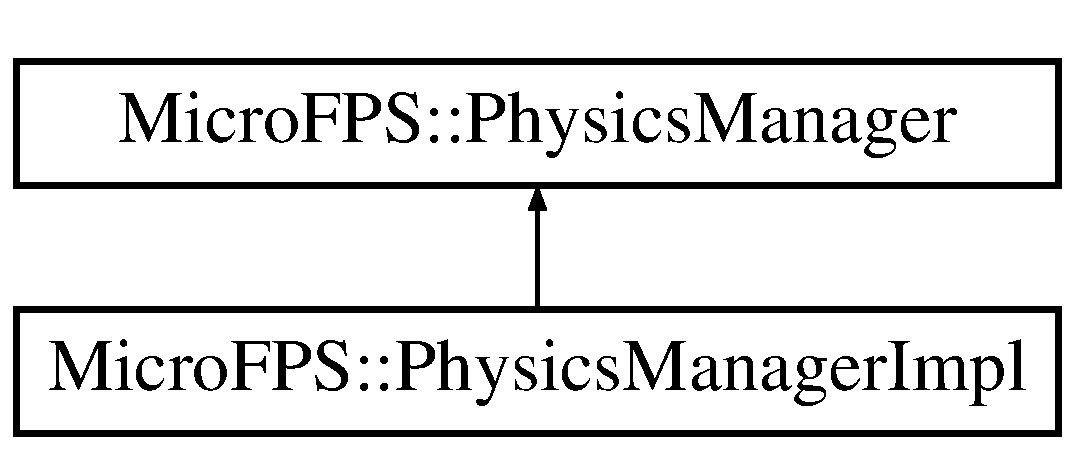
\includegraphics[height=2.000000cm]{db/d08/class_micro_f_p_s_1_1_physics_manager}
\end{center}
\end{figure}
\subsection*{Public Member Functions}
\begin{DoxyCompactItemize}
\item 
\hyperlink{class_micro_f_p_s_1_1_physics_manager_a8e7dd7b5ea2e16c07e49021f0b8e956f}{PhysicsManager} ()
\item 
virtual \hyperlink{class_micro_f_p_s_1_1_physics_manager_af11602cbafbf1d077fb04ea169629d00}{$\sim$PhysicsManager} ()
\item 
virtual physicsworld $\ast$ \hyperlink{class_micro_f_p_s_1_1_physics_manager_a3594737e8e95ffcc15e639f8cb7c7c39}{getWorld} () const =0
\item 
virtual \hyperlink{class_micro_f_p_s_1_1_physics}{Physics} $\ast$ \hyperlink{class_micro_f_p_s_1_1_physics_manager_a7983a5d70b8e47b9e0b679fc42a686a3}{getPhysicsEngine} () const =0
\end{DoxyCompactItemize}


\subsection{Detailed Description}
\hyperlink{class_micro_f_p_s_1_1_physics_manager}{PhysicsManager} Base class for physics manager 

\subsection{Constructor \& Destructor Documentation}
\hypertarget{class_micro_f_p_s_1_1_physics_manager_a8e7dd7b5ea2e16c07e49021f0b8e956f}{
\index{MicroFPS::PhysicsManager@{MicroFPS::PhysicsManager}!PhysicsManager@{PhysicsManager}}
\index{PhysicsManager@{PhysicsManager}!MicroFPS::PhysicsManager@{MicroFPS::PhysicsManager}}
\subsubsection[{PhysicsManager}]{\setlength{\rightskip}{0pt plus 5cm}MicroFPS::PhysicsManager::PhysicsManager (
\begin{DoxyParamCaption}
{}
\end{DoxyParamCaption}
)\hspace{0.3cm}{\ttfamily  \mbox{[}inline\mbox{]}}}}
\label{db/d08/class_micro_f_p_s_1_1_physics_manager_a8e7dd7b5ea2e16c07e49021f0b8e956f}
Constructor \hypertarget{class_micro_f_p_s_1_1_physics_manager_af11602cbafbf1d077fb04ea169629d00}{
\index{MicroFPS::PhysicsManager@{MicroFPS::PhysicsManager}!$\sim$PhysicsManager@{$\sim$PhysicsManager}}
\index{$\sim$PhysicsManager@{$\sim$PhysicsManager}!MicroFPS::PhysicsManager@{MicroFPS::PhysicsManager}}
\subsubsection[{$\sim$PhysicsManager}]{\setlength{\rightskip}{0pt plus 5cm}virtual MicroFPS::PhysicsManager::$\sim$PhysicsManager (
\begin{DoxyParamCaption}
{}
\end{DoxyParamCaption}
)\hspace{0.3cm}{\ttfamily  \mbox{[}inline, virtual\mbox{]}}}}
\label{db/d08/class_micro_f_p_s_1_1_physics_manager_af11602cbafbf1d077fb04ea169629d00}
Destructor 

\subsection{Member Function Documentation}
\hypertarget{class_micro_f_p_s_1_1_physics_manager_a7983a5d70b8e47b9e0b679fc42a686a3}{
\index{MicroFPS::PhysicsManager@{MicroFPS::PhysicsManager}!getPhysicsEngine@{getPhysicsEngine}}
\index{getPhysicsEngine@{getPhysicsEngine}!MicroFPS::PhysicsManager@{MicroFPS::PhysicsManager}}
\subsubsection[{getPhysicsEngine}]{\setlength{\rightskip}{0pt plus 5cm}virtual {\bf Physics}$\ast$ MicroFPS::PhysicsManager::getPhysicsEngine (
\begin{DoxyParamCaption}
{}
\end{DoxyParamCaption}
) const\hspace{0.3cm}{\ttfamily  \mbox{[}pure virtual\mbox{]}}}}
\label{db/d08/class_micro_f_p_s_1_1_physics_manager_a7983a5d70b8e47b9e0b679fc42a686a3}
\hyperlink{class_micro_f_p_s_1_1_physics_manager_a7983a5d70b8e47b9e0b679fc42a686a3}{getPhysicsEngine()} get the physics engine 

Implemented in \hyperlink{class_micro_f_p_s_1_1_physics_manager_impl_a3226e5dae46114671c03ec8d5932fe22}{MicroFPS::PhysicsManagerImpl}.

\hypertarget{class_micro_f_p_s_1_1_physics_manager_a3594737e8e95ffcc15e639f8cb7c7c39}{
\index{MicroFPS::PhysicsManager@{MicroFPS::PhysicsManager}!getWorld@{getWorld}}
\index{getWorld@{getWorld}!MicroFPS::PhysicsManager@{MicroFPS::PhysicsManager}}
\subsubsection[{getWorld}]{\setlength{\rightskip}{0pt plus 5cm}virtual physicsworld$\ast$ MicroFPS::PhysicsManager::getWorld (
\begin{DoxyParamCaption}
{}
\end{DoxyParamCaption}
) const\hspace{0.3cm}{\ttfamily  \mbox{[}pure virtual\mbox{]}}}}
\label{db/d08/class_micro_f_p_s_1_1_physics_manager_a3594737e8e95ffcc15e639f8cb7c7c39}
\hyperlink{class_micro_f_p_s_1_1_physics_manager_a3594737e8e95ffcc15e639f8cb7c7c39}{getWorld()} getPhysicsWorld 

Implemented in \hyperlink{class_micro_f_p_s_1_1_physics_manager_impl_a18cfb39e47dac9d116c9b69b1488e7e8}{MicroFPS::PhysicsManagerImpl}.



The documentation for this class was generated from the following file:\begin{DoxyCompactItemize}
\item 
C:/Users/Dennis/Desktop/MicroFPS/src/MicroFPS/src/Managers/PhysicsManager.h\end{DoxyCompactItemize}

\hypertarget{class_micro_f_p_s_1_1_physics_manager_impl}{
\section{MicroFPS::PhysicsManagerImpl Class Reference}
\label{db/d13/class_micro_f_p_s_1_1_physics_manager_impl}\index{MicroFPS::PhysicsManagerImpl@{MicroFPS::PhysicsManagerImpl}}
}
Inheritance diagram for MicroFPS::PhysicsManagerImpl:\begin{figure}[H]
\begin{center}
\leavevmode
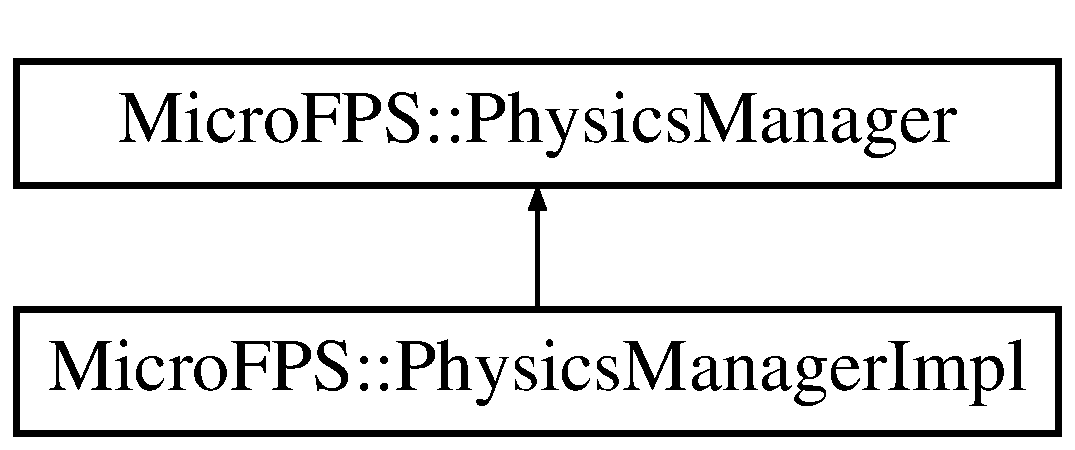
\includegraphics[height=2.000000cm]{db/d13/class_micro_f_p_s_1_1_physics_manager_impl}
\end{center}
\end{figure}
\subsection*{Public Member Functions}
\begin{DoxyCompactItemize}
\item 
\hyperlink{class_micro_f_p_s_1_1_physics_manager_impl_af09006b26f696df7b219804bc065f9f6}{PhysicsManagerImpl} ()
\item 
virtual \hyperlink{class_micro_f_p_s_1_1_physics_manager_impl_a76aea8e80f9548e9ef05a9d453b3d50f}{$\sim$PhysicsManagerImpl} ()
\item 
physicsworld $\ast$ \hyperlink{class_micro_f_p_s_1_1_physics_manager_impl_a18cfb39e47dac9d116c9b69b1488e7e8}{getWorld} () const 
\item 
\hyperlink{class_micro_f_p_s_1_1_physics}{Physics} $\ast$ \hyperlink{class_micro_f_p_s_1_1_physics_manager_impl_a3226e5dae46114671c03ec8d5932fe22}{getPhysicsEngine} () const 
\end{DoxyCompactItemize}


\subsection{Constructor \& Destructor Documentation}
\hypertarget{class_micro_f_p_s_1_1_physics_manager_impl_af09006b26f696df7b219804bc065f9f6}{
\index{MicroFPS::PhysicsManagerImpl@{MicroFPS::PhysicsManagerImpl}!PhysicsManagerImpl@{PhysicsManagerImpl}}
\index{PhysicsManagerImpl@{PhysicsManagerImpl}!MicroFPS::PhysicsManagerImpl@{MicroFPS::PhysicsManagerImpl}}
\subsubsection[{PhysicsManagerImpl}]{\setlength{\rightskip}{0pt plus 5cm}MicroFPS::PhysicsManagerImpl::PhysicsManagerImpl (
\begin{DoxyParamCaption}
{}
\end{DoxyParamCaption}
)}}
\label{db/d13/class_micro_f_p_s_1_1_physics_manager_impl_af09006b26f696df7b219804bc065f9f6}
Constructor \hypertarget{class_micro_f_p_s_1_1_physics_manager_impl_a76aea8e80f9548e9ef05a9d453b3d50f}{
\index{MicroFPS::PhysicsManagerImpl@{MicroFPS::PhysicsManagerImpl}!$\sim$PhysicsManagerImpl@{$\sim$PhysicsManagerImpl}}
\index{$\sim$PhysicsManagerImpl@{$\sim$PhysicsManagerImpl}!MicroFPS::PhysicsManagerImpl@{MicroFPS::PhysicsManagerImpl}}
\subsubsection[{$\sim$PhysicsManagerImpl}]{\setlength{\rightskip}{0pt plus 5cm}virtual MicroFPS::PhysicsManagerImpl::$\sim$PhysicsManagerImpl (
\begin{DoxyParamCaption}
{}
\end{DoxyParamCaption}
)\hspace{0.3cm}{\ttfamily  \mbox{[}virtual\mbox{]}}}}
\label{db/d13/class_micro_f_p_s_1_1_physics_manager_impl_a76aea8e80f9548e9ef05a9d453b3d50f}
Destructor 

\subsection{Member Function Documentation}
\hypertarget{class_micro_f_p_s_1_1_physics_manager_impl_a3226e5dae46114671c03ec8d5932fe22}{
\index{MicroFPS::PhysicsManagerImpl@{MicroFPS::PhysicsManagerImpl}!getPhysicsEngine@{getPhysicsEngine}}
\index{getPhysicsEngine@{getPhysicsEngine}!MicroFPS::PhysicsManagerImpl@{MicroFPS::PhysicsManagerImpl}}
\subsubsection[{getPhysicsEngine}]{\setlength{\rightskip}{0pt plus 5cm}{\bf Physics}$\ast$ MicroFPS::PhysicsManagerImpl::getPhysicsEngine (
\begin{DoxyParamCaption}
{}
\end{DoxyParamCaption}
) const\hspace{0.3cm}{\ttfamily  \mbox{[}virtual\mbox{]}}}}
\label{db/d13/class_micro_f_p_s_1_1_physics_manager_impl_a3226e5dae46114671c03ec8d5932fe22}
\hyperlink{class_micro_f_p_s_1_1_physics_manager_impl_a3226e5dae46114671c03ec8d5932fe22}{getPhysicsEngine()} 

Implements \hyperlink{class_micro_f_p_s_1_1_physics_manager_a7983a5d70b8e47b9e0b679fc42a686a3}{MicroFPS::PhysicsManager}.

\hypertarget{class_micro_f_p_s_1_1_physics_manager_impl_a18cfb39e47dac9d116c9b69b1488e7e8}{
\index{MicroFPS::PhysicsManagerImpl@{MicroFPS::PhysicsManagerImpl}!getWorld@{getWorld}}
\index{getWorld@{getWorld}!MicroFPS::PhysicsManagerImpl@{MicroFPS::PhysicsManagerImpl}}
\subsubsection[{getWorld}]{\setlength{\rightskip}{0pt plus 5cm}physicsworld$\ast$ MicroFPS::PhysicsManagerImpl::getWorld (
\begin{DoxyParamCaption}
{}
\end{DoxyParamCaption}
) const\hspace{0.3cm}{\ttfamily  \mbox{[}virtual\mbox{]}}}}
\label{db/d13/class_micro_f_p_s_1_1_physics_manager_impl_a18cfb39e47dac9d116c9b69b1488e7e8}
\hyperlink{class_micro_f_p_s_1_1_physics_manager_impl_a18cfb39e47dac9d116c9b69b1488e7e8}{getWorld()} 

Implements \hyperlink{class_micro_f_p_s_1_1_physics_manager_a3594737e8e95ffcc15e639f8cb7c7c39}{MicroFPS::PhysicsManager}.



The documentation for this class was generated from the following file:\begin{DoxyCompactItemize}
\item 
C:/Users/Dennis/Desktop/MicroFPS/src/MicroFPS/src/Impl/PhysicsManagerImpl.h\end{DoxyCompactItemize}

\hypertarget{class_micro_f_p_s_1_1_renderer}{
\section{MicroFPS::Renderer Class Reference}
\label{d6/de2/class_micro_f_p_s_1_1_renderer}\index{MicroFPS::Renderer@{MicroFPS::Renderer}}
}


{\ttfamily \#include $<$Renderer.h$>$}

Inheritance diagram for MicroFPS::Renderer:\begin{figure}[H]
\begin{center}
\leavevmode
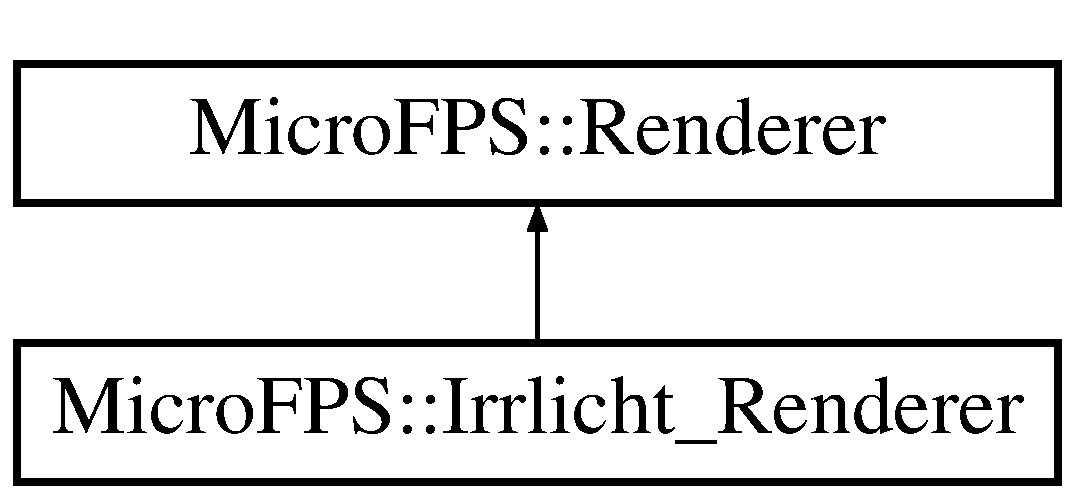
\includegraphics[height=2.000000cm]{d6/de2/class_micro_f_p_s_1_1_renderer}
\end{center}
\end{figure}
\subsection*{Public Member Functions}
\begin{DoxyCompactItemize}
\item 
\hyperlink{class_micro_f_p_s_1_1_renderer_a6e485790e7feded6cda1c6c69cf20940}{Renderer} ()
\item 
virtual \hyperlink{class_micro_f_p_s_1_1_renderer_a89ef8839d0624fc08d55bcad40a4898d}{$\sim$Renderer} ()
\item 
virtual renderer \hyperlink{class_micro_f_p_s_1_1_renderer_a092a7585391cd2a6067c80d8d989e8dd}{getRendererDevice} () const =0
\item 
virtual void \hyperlink{class_micro_f_p_s_1_1_renderer_a855df0a5be7f49d50f5de6be106376c3}{gameLoop} ()=0
\end{DoxyCompactItemize}


\subsection{Detailed Description}
\hyperlink{class_micro_f_p_s_1_1_renderer}{Renderer} Base class for all renderer connectors 

\subsection{Constructor \& Destructor Documentation}
\hypertarget{class_micro_f_p_s_1_1_renderer_a6e485790e7feded6cda1c6c69cf20940}{
\index{MicroFPS::Renderer@{MicroFPS::Renderer}!Renderer@{Renderer}}
\index{Renderer@{Renderer}!MicroFPS::Renderer@{MicroFPS::Renderer}}
\subsubsection[{Renderer}]{\setlength{\rightskip}{0pt plus 5cm}MicroFPS::Renderer::Renderer (
\begin{DoxyParamCaption}
{}
\end{DoxyParamCaption}
)\hspace{0.3cm}{\ttfamily  \mbox{[}inline\mbox{]}}}}
\label{d6/de2/class_micro_f_p_s_1_1_renderer_a6e485790e7feded6cda1c6c69cf20940}
Constructor \hypertarget{class_micro_f_p_s_1_1_renderer_a89ef8839d0624fc08d55bcad40a4898d}{
\index{MicroFPS::Renderer@{MicroFPS::Renderer}!$\sim$Renderer@{$\sim$Renderer}}
\index{$\sim$Renderer@{$\sim$Renderer}!MicroFPS::Renderer@{MicroFPS::Renderer}}
\subsubsection[{$\sim$Renderer}]{\setlength{\rightskip}{0pt plus 5cm}virtual MicroFPS::Renderer::$\sim$Renderer (
\begin{DoxyParamCaption}
{}
\end{DoxyParamCaption}
)\hspace{0.3cm}{\ttfamily  \mbox{[}inline, virtual\mbox{]}}}}
\label{d6/de2/class_micro_f_p_s_1_1_renderer_a89ef8839d0624fc08d55bcad40a4898d}
Destructor 

\subsection{Member Function Documentation}
\hypertarget{class_micro_f_p_s_1_1_renderer_a855df0a5be7f49d50f5de6be106376c3}{
\index{MicroFPS::Renderer@{MicroFPS::Renderer}!gameLoop@{gameLoop}}
\index{gameLoop@{gameLoop}!MicroFPS::Renderer@{MicroFPS::Renderer}}
\subsubsection[{gameLoop}]{\setlength{\rightskip}{0pt plus 5cm}virtual void MicroFPS::Renderer::gameLoop (
\begin{DoxyParamCaption}
{}
\end{DoxyParamCaption}
)\hspace{0.3cm}{\ttfamily  \mbox{[}pure virtual\mbox{]}}}}
\label{d6/de2/class_micro_f_p_s_1_1_renderer_a855df0a5be7f49d50f5de6be106376c3}
gameLoop Define the game loop method for this engine 

Implemented in \hyperlink{class_micro_f_p_s_1_1_irrlicht___renderer_ac719b88be714f1ece203d6dc3cce7ae2}{MicroFPS::Irrlicht\_\-Renderer}.

\hypertarget{class_micro_f_p_s_1_1_renderer_a092a7585391cd2a6067c80d8d989e8dd}{
\index{MicroFPS::Renderer@{MicroFPS::Renderer}!getRendererDevice@{getRendererDevice}}
\index{getRendererDevice@{getRendererDevice}!MicroFPS::Renderer@{MicroFPS::Renderer}}
\subsubsection[{getRendererDevice}]{\setlength{\rightskip}{0pt plus 5cm}virtual renderer MicroFPS::Renderer::getRendererDevice (
\begin{DoxyParamCaption}
{}
\end{DoxyParamCaption}
) const\hspace{0.3cm}{\ttfamily  \mbox{[}pure virtual\mbox{]}}}}
\label{d6/de2/class_micro_f_p_s_1_1_renderer_a092a7585391cd2a6067c80d8d989e8dd}
getRendererDevice Create the render device for this engine 

Implemented in \hyperlink{class_micro_f_p_s_1_1_irrlicht___renderer_a6150c60d9599047f2d0ce468d4b3ac56}{MicroFPS::Irrlicht\_\-Renderer}.



The documentation for this class was generated from the following file:\begin{DoxyCompactItemize}
\item 
C:/Users/Dennis/Desktop/MicroFPS/src/MicroFPS/src/RenderEngines/Renderer.h\end{DoxyCompactItemize}

\hypertarget{class_micro_f_p_s_1_1_render_manager}{
\section{MicroFPS::RenderManager Class Reference}
\label{d2/dad/class_micro_f_p_s_1_1_render_manager}\index{MicroFPS::RenderManager@{MicroFPS::RenderManager}}
}
Inheritance diagram for MicroFPS::RenderManager:\begin{figure}[H]
\begin{center}
\leavevmode
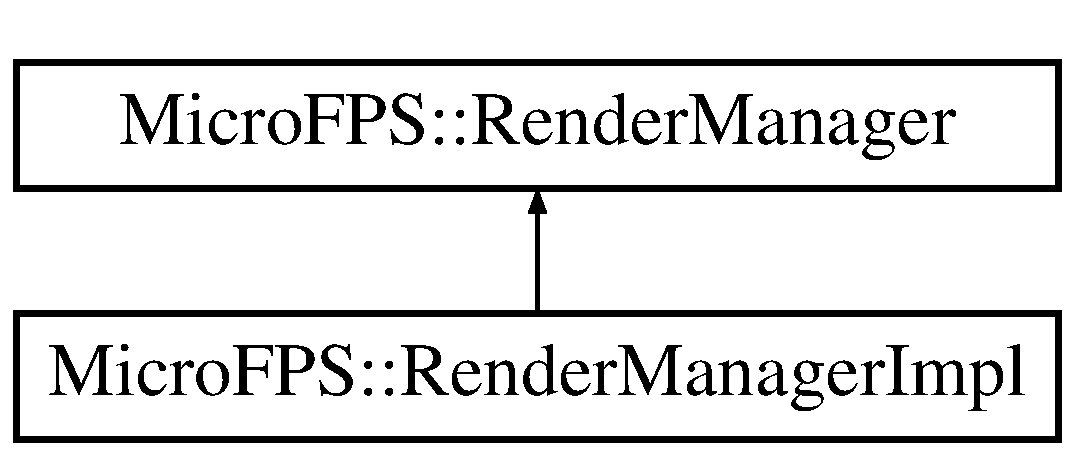
\includegraphics[height=2.000000cm]{d2/dad/class_micro_f_p_s_1_1_render_manager}
\end{center}
\end{figure}
\subsection*{Public Member Functions}
\begin{DoxyCompactItemize}
\item 
\hyperlink{class_micro_f_p_s_1_1_render_manager_aa5cfdf42a7aeed598d8cd6b406ba2224}{RenderManager} ()
\item 
virtual \hyperlink{class_micro_f_p_s_1_1_render_manager_aee2394d07bc912d3165fe4dbd4a456dd}{$\sim$RenderManager} ()
\item 
virtual renderer \hyperlink{class_micro_f_p_s_1_1_render_manager_acb0e88bc424463200c4bdf451ea3c3ad}{getRenderDevice} () const =0
\item 
virtual bool \hyperlink{class_micro_f_p_s_1_1_render_manager_a32778d202b6dcde145be54846a6a9a64}{loop} () const =0
\item 
virtual void \hyperlink{class_micro_f_p_s_1_1_render_manager_af258ceee6bf336eaf765c9178ef5becc}{gameLoop} (\hyperlink{class_micro_f_p_s_1_1_game_state}{GameState} $\ast$state=0)=0
\end{DoxyCompactItemize}


\subsection{Constructor \& Destructor Documentation}
\hypertarget{class_micro_f_p_s_1_1_render_manager_aa5cfdf42a7aeed598d8cd6b406ba2224}{
\index{MicroFPS::RenderManager@{MicroFPS::RenderManager}!RenderManager@{RenderManager}}
\index{RenderManager@{RenderManager}!MicroFPS::RenderManager@{MicroFPS::RenderManager}}
\subsubsection[{RenderManager}]{\setlength{\rightskip}{0pt plus 5cm}MicroFPS::RenderManager::RenderManager (
\begin{DoxyParamCaption}
{}
\end{DoxyParamCaption}
)\hspace{0.3cm}{\ttfamily  \mbox{[}inline\mbox{]}}}}
\label{d2/dad/class_micro_f_p_s_1_1_render_manager_aa5cfdf42a7aeed598d8cd6b406ba2224}
\hyperlink{class_micro_f_p_s_1_1_render_manager_aa5cfdf42a7aeed598d8cd6b406ba2224}{RenderManager()} Default constructor \hypertarget{class_micro_f_p_s_1_1_render_manager_aee2394d07bc912d3165fe4dbd4a456dd}{
\index{MicroFPS::RenderManager@{MicroFPS::RenderManager}!$\sim$RenderManager@{$\sim$RenderManager}}
\index{$\sim$RenderManager@{$\sim$RenderManager}!MicroFPS::RenderManager@{MicroFPS::RenderManager}}
\subsubsection[{$\sim$RenderManager}]{\setlength{\rightskip}{0pt plus 5cm}virtual MicroFPS::RenderManager::$\sim$RenderManager (
\begin{DoxyParamCaption}
{}
\end{DoxyParamCaption}
)\hspace{0.3cm}{\ttfamily  \mbox{[}inline, virtual\mbox{]}}}}
\label{d2/dad/class_micro_f_p_s_1_1_render_manager_aee2394d07bc912d3165fe4dbd4a456dd}
\hyperlink{class_micro_f_p_s_1_1_render_manager_aee2394d07bc912d3165fe4dbd4a456dd}{$\sim$RenderManager()} virtual destructor 

\subsection{Member Function Documentation}
\hypertarget{class_micro_f_p_s_1_1_render_manager_af258ceee6bf336eaf765c9178ef5becc}{
\index{MicroFPS::RenderManager@{MicroFPS::RenderManager}!gameLoop@{gameLoop}}
\index{gameLoop@{gameLoop}!MicroFPS::RenderManager@{MicroFPS::RenderManager}}
\subsubsection[{gameLoop}]{\setlength{\rightskip}{0pt plus 5cm}virtual void MicroFPS::RenderManager::gameLoop (
\begin{DoxyParamCaption}
\item[{{\bf GameState} $\ast$}]{state = {\ttfamily 0}}
\end{DoxyParamCaption}
)\hspace{0.3cm}{\ttfamily  \mbox{[}pure virtual\mbox{]}}}}
\label{d2/dad/class_micro_f_p_s_1_1_render_manager_af258ceee6bf336eaf765c9178ef5becc}
gameLoop Get game loop 

Implemented in \hyperlink{class_micro_f_p_s_1_1_render_manager_impl_a5967f1a8917ea93a5e9a1fd4ec2beedc}{MicroFPS::RenderManagerImpl}.

\hypertarget{class_micro_f_p_s_1_1_render_manager_acb0e88bc424463200c4bdf451ea3c3ad}{
\index{MicroFPS::RenderManager@{MicroFPS::RenderManager}!getRenderDevice@{getRenderDevice}}
\index{getRenderDevice@{getRenderDevice}!MicroFPS::RenderManager@{MicroFPS::RenderManager}}
\subsubsection[{getRenderDevice}]{\setlength{\rightskip}{0pt plus 5cm}virtual renderer MicroFPS::RenderManager::getRenderDevice (
\begin{DoxyParamCaption}
{}
\end{DoxyParamCaption}
) const\hspace{0.3cm}{\ttfamily  \mbox{[}pure virtual\mbox{]}}}}
\label{d2/dad/class_micro_f_p_s_1_1_render_manager_acb0e88bc424463200c4bdf451ea3c3ad}
getRenderDevice Retrieves the render device for the game 

Implemented in \hyperlink{class_micro_f_p_s_1_1_render_manager_impl_ae20d62f6586e0b9fd2513d7b880f65fc}{MicroFPS::RenderManagerImpl}.

\hypertarget{class_micro_f_p_s_1_1_render_manager_a32778d202b6dcde145be54846a6a9a64}{
\index{MicroFPS::RenderManager@{MicroFPS::RenderManager}!loop@{loop}}
\index{loop@{loop}!MicroFPS::RenderManager@{MicroFPS::RenderManager}}
\subsubsection[{loop}]{\setlength{\rightskip}{0pt plus 5cm}virtual bool MicroFPS::RenderManager::loop (
\begin{DoxyParamCaption}
{}
\end{DoxyParamCaption}
) const\hspace{0.3cm}{\ttfamily  \mbox{[}pure virtual\mbox{]}}}}
\label{d2/dad/class_micro_f_p_s_1_1_render_manager_a32778d202b6dcde145be54846a6a9a64}
loop Determine whether to continue looping or not 

Implemented in \hyperlink{class_micro_f_p_s_1_1_render_manager_impl_afa5e1bcacb69beb73f00701db08769d2}{MicroFPS::RenderManagerImpl}.



The documentation for this class was generated from the following file:\begin{DoxyCompactItemize}
\item 
C:/Users/Dennis/Desktop/MicroFPS/src/MicroFPS/src/Managers/RenderManager.h\end{DoxyCompactItemize}

\hypertarget{class_micro_f_p_s_1_1_render_manager_impl}{
\section{MicroFPS::RenderManagerImpl Class Reference}
\label{de/d41/class_micro_f_p_s_1_1_render_manager_impl}\index{MicroFPS::RenderManagerImpl@{MicroFPS::RenderManagerImpl}}
}
Inheritance diagram for MicroFPS::RenderManagerImpl:\begin{figure}[H]
\begin{center}
\leavevmode
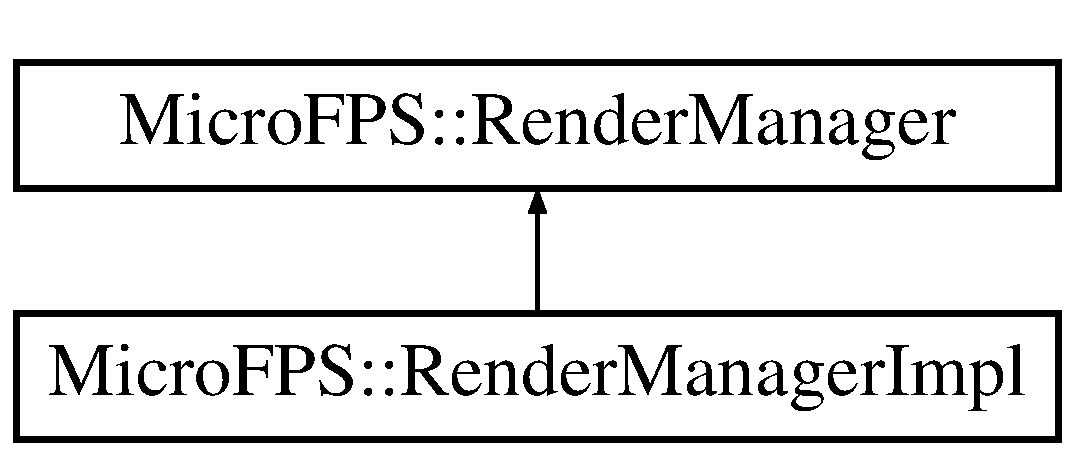
\includegraphics[height=2.000000cm]{de/d41/class_micro_f_p_s_1_1_render_manager_impl}
\end{center}
\end{figure}
\subsection*{Public Member Functions}
\begin{DoxyCompactItemize}
\item 
\hyperlink{class_micro_f_p_s_1_1_render_manager_impl_a3fe0b36c083e52153d4118c7e68ec842}{RenderManagerImpl} ()
\item 
virtual \hyperlink{class_micro_f_p_s_1_1_render_manager_impl_a4e64d05f033e969f4d73369ff85ffabe}{$\sim$RenderManagerImpl} ()
\item 
virtual renderer \hyperlink{class_micro_f_p_s_1_1_render_manager_impl_ae20d62f6586e0b9fd2513d7b880f65fc}{getRenderDevice} () const 
\item 
virtual bool \hyperlink{class_micro_f_p_s_1_1_render_manager_impl_afa5e1bcacb69beb73f00701db08769d2}{loop} () const 
\item 
virtual void \hyperlink{class_micro_f_p_s_1_1_render_manager_impl_a5967f1a8917ea93a5e9a1fd4ec2beedc}{gameLoop} (\hyperlink{class_micro_f_p_s_1_1_game_state}{GameState} $\ast$state=0)
\end{DoxyCompactItemize}


\subsection{Constructor \& Destructor Documentation}
\hypertarget{class_micro_f_p_s_1_1_render_manager_impl_a3fe0b36c083e52153d4118c7e68ec842}{
\index{MicroFPS::RenderManagerImpl@{MicroFPS::RenderManagerImpl}!RenderManagerImpl@{RenderManagerImpl}}
\index{RenderManagerImpl@{RenderManagerImpl}!MicroFPS::RenderManagerImpl@{MicroFPS::RenderManagerImpl}}
\subsubsection[{RenderManagerImpl}]{\setlength{\rightskip}{0pt plus 5cm}MicroFPS::RenderManagerImpl::RenderManagerImpl (
\begin{DoxyParamCaption}
{}
\end{DoxyParamCaption}
)}}
\label{de/d41/class_micro_f_p_s_1_1_render_manager_impl_a3fe0b36c083e52153d4118c7e68ec842}
Constructor \hypertarget{class_micro_f_p_s_1_1_render_manager_impl_a4e64d05f033e969f4d73369ff85ffabe}{
\index{MicroFPS::RenderManagerImpl@{MicroFPS::RenderManagerImpl}!$\sim$RenderManagerImpl@{$\sim$RenderManagerImpl}}
\index{$\sim$RenderManagerImpl@{$\sim$RenderManagerImpl}!MicroFPS::RenderManagerImpl@{MicroFPS::RenderManagerImpl}}
\subsubsection[{$\sim$RenderManagerImpl}]{\setlength{\rightskip}{0pt plus 5cm}virtual MicroFPS::RenderManagerImpl::$\sim$RenderManagerImpl (
\begin{DoxyParamCaption}
{}
\end{DoxyParamCaption}
)\hspace{0.3cm}{\ttfamily  \mbox{[}virtual\mbox{]}}}}
\label{de/d41/class_micro_f_p_s_1_1_render_manager_impl_a4e64d05f033e969f4d73369ff85ffabe}
Destructor
\begin{DoxyItemize}
\item Don't leak $<$3 
\end{DoxyItemize}

\subsection{Member Function Documentation}
\hypertarget{class_micro_f_p_s_1_1_render_manager_impl_a5967f1a8917ea93a5e9a1fd4ec2beedc}{
\index{MicroFPS::RenderManagerImpl@{MicroFPS::RenderManagerImpl}!gameLoop@{gameLoop}}
\index{gameLoop@{gameLoop}!MicroFPS::RenderManagerImpl@{MicroFPS::RenderManagerImpl}}
\subsubsection[{gameLoop}]{\setlength{\rightskip}{0pt plus 5cm}virtual void MicroFPS::RenderManagerImpl::gameLoop (
\begin{DoxyParamCaption}
\item[{{\bf GameState} $\ast$}]{state = {\ttfamily 0}}
\end{DoxyParamCaption}
)\hspace{0.3cm}{\ttfamily  \mbox{[}virtual\mbox{]}}}}
\label{de/d41/class_micro_f_p_s_1_1_render_manager_impl_a5967f1a8917ea93a5e9a1fd4ec2beedc}
gameLoop Run the game loop 

Implements \hyperlink{class_micro_f_p_s_1_1_render_manager_af258ceee6bf336eaf765c9178ef5becc}{MicroFPS::RenderManager}.

\hypertarget{class_micro_f_p_s_1_1_render_manager_impl_ae20d62f6586e0b9fd2513d7b880f65fc}{
\index{MicroFPS::RenderManagerImpl@{MicroFPS::RenderManagerImpl}!getRenderDevice@{getRenderDevice}}
\index{getRenderDevice@{getRenderDevice}!MicroFPS::RenderManagerImpl@{MicroFPS::RenderManagerImpl}}
\subsubsection[{getRenderDevice}]{\setlength{\rightskip}{0pt plus 5cm}virtual renderer MicroFPS::RenderManagerImpl::getRenderDevice (
\begin{DoxyParamCaption}
{}
\end{DoxyParamCaption}
) const\hspace{0.3cm}{\ttfamily  \mbox{[}virtual\mbox{]}}}}
\label{de/d41/class_micro_f_p_s_1_1_render_manager_impl_ae20d62f6586e0b9fd2513d7b880f65fc}
getRenderDevice Get the current rendering device \begin{DoxyReturn}{Returns}
renderer device (renderer varies based on specific configuration) 
\end{DoxyReturn}


Implements \hyperlink{class_micro_f_p_s_1_1_render_manager_acb0e88bc424463200c4bdf451ea3c3ad}{MicroFPS::RenderManager}.

\hypertarget{class_micro_f_p_s_1_1_render_manager_impl_afa5e1bcacb69beb73f00701db08769d2}{
\index{MicroFPS::RenderManagerImpl@{MicroFPS::RenderManagerImpl}!loop@{loop}}
\index{loop@{loop}!MicroFPS::RenderManagerImpl@{MicroFPS::RenderManagerImpl}}
\subsubsection[{loop}]{\setlength{\rightskip}{0pt plus 5cm}virtual bool MicroFPS::RenderManagerImpl::loop (
\begin{DoxyParamCaption}
{}
\end{DoxyParamCaption}
) const\hspace{0.3cm}{\ttfamily  \mbox{[}virtual\mbox{]}}}}
\label{de/d41/class_micro_f_p_s_1_1_render_manager_impl_afa5e1bcacb69beb73f00701db08769d2}
loop Determine whether to continue looping or not 

Implements \hyperlink{class_micro_f_p_s_1_1_render_manager_a32778d202b6dcde145be54846a6a9a64}{MicroFPS::RenderManager}.



The documentation for this class was generated from the following file:\begin{DoxyCompactItemize}
\item 
C:/Users/Dennis/Desktop/MicroFPS/src/MicroFPS/src/Impl/RenderManagerImpl.h\end{DoxyCompactItemize}

\hypertarget{class_micro_f_p_s_1_1_state_manager}{
\section{MicroFPS::StateManager Class Reference}
\label{d2/dbd/class_micro_f_p_s_1_1_state_manager}\index{MicroFPS::StateManager@{MicroFPS::StateManager}}
}


{\ttfamily \#include $<$StateManager.h$>$}

Inheritance diagram for MicroFPS::StateManager:\begin{figure}[H]
\begin{center}
\leavevmode
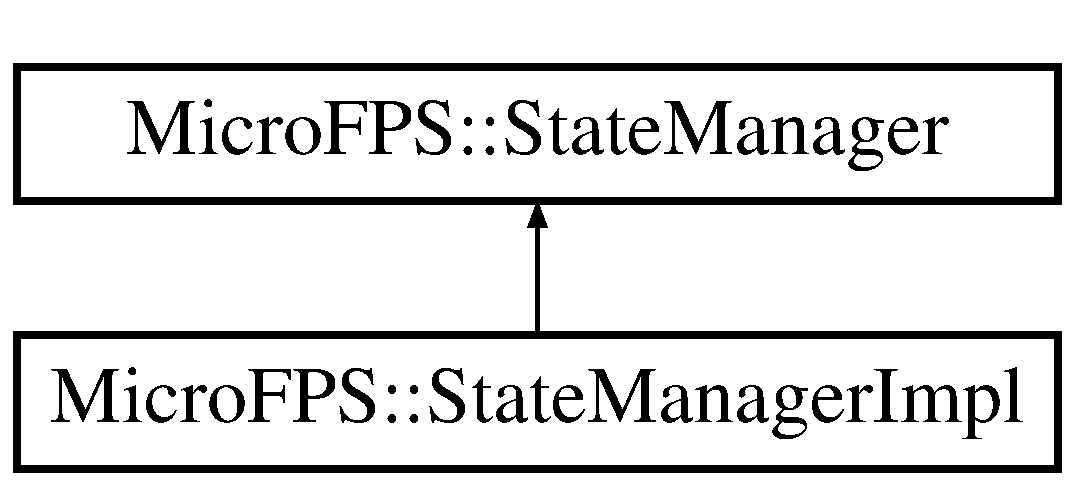
\includegraphics[height=2.000000cm]{d2/dbd/class_micro_f_p_s_1_1_state_manager}
\end{center}
\end{figure}
\subsection*{Public Member Functions}
\begin{DoxyCompactItemize}
\item 
\hyperlink{class_micro_f_p_s_1_1_state_manager_a05450ac05314e7f0ca504c814809ba32}{StateManager} ()
\item 
virtual \hyperlink{class_micro_f_p_s_1_1_state_manager_ab07b0637b6730764afd561a9cae29b02}{$\sim$StateManager} ()
\item 
virtual \hyperlink{class_micro_f_p_s_1_1_game_state}{GameState} $\ast$ \hyperlink{class_micro_f_p_s_1_1_state_manager_ac7399e6e56923dd9b45e3ae1169b55f7}{getCurrentState} () const =0
\item 
virtual void \hyperlink{class_micro_f_p_s_1_1_state_manager_a6fe3b8c2c4cc7f577438c5b1595d973c}{setCurrentState} (std::string state)=0
\item 
virtual void \hyperlink{class_micro_f_p_s_1_1_state_manager_ac0d581ea9f4e2d1f15055a3cf749508a}{addState} (std::string name, \hyperlink{class_micro_f_p_s_1_1_game_state}{GameState} $\ast$state)=0
\item 
virtual void \hyperlink{class_micro_f_p_s_1_1_state_manager_a19423bbbfcdc714c176e0be4073355f0}{removeState} (std::string state)=0
\item 
virtual GUI $\ast$ \hyperlink{class_micro_f_p_s_1_1_state_manager_a87e67ff37f90da0d9ad15a8411f98d69}{getGUI} () const =0
\end{DoxyCompactItemize}


\subsection{Detailed Description}
\hyperlink{class_micro_f_p_s_1_1_state_manager}{StateManager} Abstract class for state management 

\subsection{Constructor \& Destructor Documentation}
\hypertarget{class_micro_f_p_s_1_1_state_manager_a05450ac05314e7f0ca504c814809ba32}{
\index{MicroFPS::StateManager@{MicroFPS::StateManager}!StateManager@{StateManager}}
\index{StateManager@{StateManager}!MicroFPS::StateManager@{MicroFPS::StateManager}}
\subsubsection[{StateManager}]{\setlength{\rightskip}{0pt plus 5cm}MicroFPS::StateManager::StateManager (
\begin{DoxyParamCaption}
{}
\end{DoxyParamCaption}
)\hspace{0.3cm}{\ttfamily  \mbox{[}inline\mbox{]}}}}
\label{d2/dbd/class_micro_f_p_s_1_1_state_manager_a05450ac05314e7f0ca504c814809ba32}
Constructor \hypertarget{class_micro_f_p_s_1_1_state_manager_ab07b0637b6730764afd561a9cae29b02}{
\index{MicroFPS::StateManager@{MicroFPS::StateManager}!$\sim$StateManager@{$\sim$StateManager}}
\index{$\sim$StateManager@{$\sim$StateManager}!MicroFPS::StateManager@{MicroFPS::StateManager}}
\subsubsection[{$\sim$StateManager}]{\setlength{\rightskip}{0pt plus 5cm}virtual MicroFPS::StateManager::$\sim$StateManager (
\begin{DoxyParamCaption}
{}
\end{DoxyParamCaption}
)\hspace{0.3cm}{\ttfamily  \mbox{[}inline, virtual\mbox{]}}}}
\label{d2/dbd/class_micro_f_p_s_1_1_state_manager_ab07b0637b6730764afd561a9cae29b02}
Destructor 

\subsection{Member Function Documentation}
\hypertarget{class_micro_f_p_s_1_1_state_manager_ac0d581ea9f4e2d1f15055a3cf749508a}{
\index{MicroFPS::StateManager@{MicroFPS::StateManager}!addState@{addState}}
\index{addState@{addState}!MicroFPS::StateManager@{MicroFPS::StateManager}}
\subsubsection[{addState}]{\setlength{\rightskip}{0pt plus 5cm}virtual void MicroFPS::StateManager::addState (
\begin{DoxyParamCaption}
\item[{std::string}]{name, }
\item[{{\bf GameState} $\ast$}]{state}
\end{DoxyParamCaption}
)\hspace{0.3cm}{\ttfamily  \mbox{[}pure virtual\mbox{]}}}}
\label{d2/dbd/class_micro_f_p_s_1_1_state_manager_ac0d581ea9f4e2d1f15055a3cf749508a}
addState Add a new state to the state manager 

Implemented in \hyperlink{class_micro_f_p_s_1_1_state_manager_impl_a8fffe04cfd95c1f84989a99b34e29ba2}{MicroFPS::StateManagerImpl}.

\hypertarget{class_micro_f_p_s_1_1_state_manager_ac7399e6e56923dd9b45e3ae1169b55f7}{
\index{MicroFPS::StateManager@{MicroFPS::StateManager}!getCurrentState@{getCurrentState}}
\index{getCurrentState@{getCurrentState}!MicroFPS::StateManager@{MicroFPS::StateManager}}
\subsubsection[{getCurrentState}]{\setlength{\rightskip}{0pt plus 5cm}virtual {\bf GameState}$\ast$ MicroFPS::StateManager::getCurrentState (
\begin{DoxyParamCaption}
{}
\end{DoxyParamCaption}
) const\hspace{0.3cm}{\ttfamily  \mbox{[}pure virtual\mbox{]}}}}
\label{d2/dbd/class_micro_f_p_s_1_1_state_manager_ac7399e6e56923dd9b45e3ae1169b55f7}
getCurrentState Get the current game state 

Implemented in \hyperlink{class_micro_f_p_s_1_1_state_manager_impl_aed21558f8d76cd3dce1a9fc5f76ea3c8}{MicroFPS::StateManagerImpl}.

\hypertarget{class_micro_f_p_s_1_1_state_manager_a87e67ff37f90da0d9ad15a8411f98d69}{
\index{MicroFPS::StateManager@{MicroFPS::StateManager}!getGUI@{getGUI}}
\index{getGUI@{getGUI}!MicroFPS::StateManager@{MicroFPS::StateManager}}
\subsubsection[{getGUI}]{\setlength{\rightskip}{0pt plus 5cm}virtual GUI$\ast$ MicroFPS::StateManager::getGUI (
\begin{DoxyParamCaption}
{}
\end{DoxyParamCaption}
) const\hspace{0.3cm}{\ttfamily  \mbox{[}pure virtual\mbox{]}}}}
\label{d2/dbd/class_micro_f_p_s_1_1_state_manager_a87e67ff37f90da0d9ad15a8411f98d69}
getGUI Get GUI pointer 

Implemented in \hyperlink{class_micro_f_p_s_1_1_state_manager_impl_aeb4fcc00613a7c42376e6afb76b14b54}{MicroFPS::StateManagerImpl}.

\hypertarget{class_micro_f_p_s_1_1_state_manager_a19423bbbfcdc714c176e0be4073355f0}{
\index{MicroFPS::StateManager@{MicroFPS::StateManager}!removeState@{removeState}}
\index{removeState@{removeState}!MicroFPS::StateManager@{MicroFPS::StateManager}}
\subsubsection[{removeState}]{\setlength{\rightskip}{0pt plus 5cm}virtual void MicroFPS::StateManager::removeState (
\begin{DoxyParamCaption}
\item[{std::string}]{state}
\end{DoxyParamCaption}
)\hspace{0.3cm}{\ttfamily  \mbox{[}pure virtual\mbox{]}}}}
\label{d2/dbd/class_micro_f_p_s_1_1_state_manager_a19423bbbfcdc714c176e0be4073355f0}
removeState Remove a particular state from the state manager 

Implemented in \hyperlink{class_micro_f_p_s_1_1_state_manager_impl_aefaa0295e49d20310bd2e95212aaa091}{MicroFPS::StateManagerImpl}.

\hypertarget{class_micro_f_p_s_1_1_state_manager_a6fe3b8c2c4cc7f577438c5b1595d973c}{
\index{MicroFPS::StateManager@{MicroFPS::StateManager}!setCurrentState@{setCurrentState}}
\index{setCurrentState@{setCurrentState}!MicroFPS::StateManager@{MicroFPS::StateManager}}
\subsubsection[{setCurrentState}]{\setlength{\rightskip}{0pt plus 5cm}virtual void MicroFPS::StateManager::setCurrentState (
\begin{DoxyParamCaption}
\item[{std::string}]{state}
\end{DoxyParamCaption}
)\hspace{0.3cm}{\ttfamily  \mbox{[}pure virtual\mbox{]}}}}
\label{d2/dbd/class_micro_f_p_s_1_1_state_manager_a6fe3b8c2c4cc7f577438c5b1595d973c}
setCurrentState Change the game state 

Implemented in \hyperlink{class_micro_f_p_s_1_1_state_manager_impl_a36be818e3d8b561ef9372a1e043c05ed}{MicroFPS::StateManagerImpl}.



The documentation for this class was generated from the following file:\begin{DoxyCompactItemize}
\item 
C:/Users/Dennis/Desktop/MicroFPS/src/MicroFPS/src/Managers/StateManager.h\end{DoxyCompactItemize}

\hypertarget{class_micro_f_p_s_1_1_state_manager_impl}{
\section{MicroFPS::StateManagerImpl Class Reference}
\label{d9/dc7/class_micro_f_p_s_1_1_state_manager_impl}\index{MicroFPS::StateManagerImpl@{MicroFPS::StateManagerImpl}}
}


{\ttfamily \#include $<$StateManagerImpl.h$>$}

Inheritance diagram for MicroFPS::StateManagerImpl:\begin{figure}[H]
\begin{center}
\leavevmode
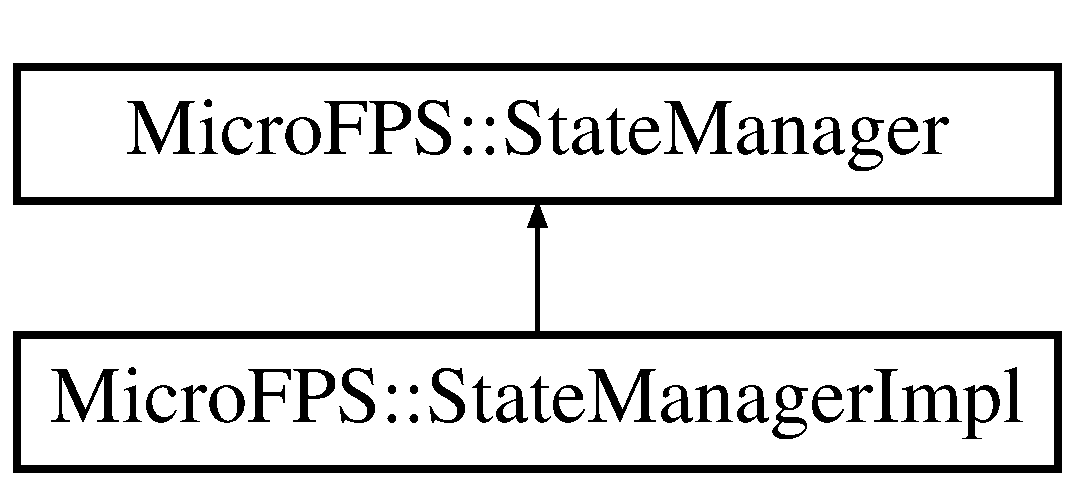
\includegraphics[height=2.000000cm]{d9/dc7/class_micro_f_p_s_1_1_state_manager_impl}
\end{center}
\end{figure}
\subsection*{Public Member Functions}
\begin{DoxyCompactItemize}
\item 
\hyperlink{class_micro_f_p_s_1_1_state_manager_impl_a5b0fd02ecf88778548542bf58f4e75bc}{StateManagerImpl} (renderer device)
\item 
virtual \hyperlink{class_micro_f_p_s_1_1_state_manager_impl_a6f244e71038028b079f301ad98a23266}{$\sim$StateManagerImpl} ()
\item 
virtual \hyperlink{class_micro_f_p_s_1_1_game_state}{GameState} $\ast$ \hyperlink{class_micro_f_p_s_1_1_state_manager_impl_aed21558f8d76cd3dce1a9fc5f76ea3c8}{getCurrentState} () const 
\item 
virtual void \hyperlink{class_micro_f_p_s_1_1_state_manager_impl_a36be818e3d8b561ef9372a1e043c05ed}{setCurrentState} (std::string state)
\item 
virtual void \hyperlink{class_micro_f_p_s_1_1_state_manager_impl_a8fffe04cfd95c1f84989a99b34e29ba2}{addState} (std::string name, \hyperlink{class_micro_f_p_s_1_1_game_state}{GameState} $\ast$state)
\item 
virtual void \hyperlink{class_micro_f_p_s_1_1_state_manager_impl_aefaa0295e49d20310bd2e95212aaa091}{removeState} (std::string state)
\item 
virtual GUI $\ast$ \hyperlink{class_micro_f_p_s_1_1_state_manager_impl_aeb4fcc00613a7c42376e6afb76b14b54}{getGUI} () const 
\end{DoxyCompactItemize}


\subsection{Detailed Description}
\hyperlink{class_micro_f_p_s_1_1_state_manager_impl}{StateManagerImpl} Implementation for state manager 

\subsection{Constructor \& Destructor Documentation}
\hypertarget{class_micro_f_p_s_1_1_state_manager_impl_a5b0fd02ecf88778548542bf58f4e75bc}{
\index{MicroFPS::StateManagerImpl@{MicroFPS::StateManagerImpl}!StateManagerImpl@{StateManagerImpl}}
\index{StateManagerImpl@{StateManagerImpl}!MicroFPS::StateManagerImpl@{MicroFPS::StateManagerImpl}}
\subsubsection[{StateManagerImpl}]{\setlength{\rightskip}{0pt plus 5cm}MicroFPS::StateManagerImpl::StateManagerImpl (
\begin{DoxyParamCaption}
\item[{renderer}]{device}
\end{DoxyParamCaption}
)}}
\label{d9/dc7/class_micro_f_p_s_1_1_state_manager_impl_a5b0fd02ecf88778548542bf58f4e75bc}
Constructor \hypertarget{class_micro_f_p_s_1_1_state_manager_impl_a6f244e71038028b079f301ad98a23266}{
\index{MicroFPS::StateManagerImpl@{MicroFPS::StateManagerImpl}!$\sim$StateManagerImpl@{$\sim$StateManagerImpl}}
\index{$\sim$StateManagerImpl@{$\sim$StateManagerImpl}!MicroFPS::StateManagerImpl@{MicroFPS::StateManagerImpl}}
\subsubsection[{$\sim$StateManagerImpl}]{\setlength{\rightskip}{0pt plus 5cm}virtual MicroFPS::StateManagerImpl::$\sim$StateManagerImpl (
\begin{DoxyParamCaption}
{}
\end{DoxyParamCaption}
)\hspace{0.3cm}{\ttfamily  \mbox{[}virtual\mbox{]}}}}
\label{d9/dc7/class_micro_f_p_s_1_1_state_manager_impl_a6f244e71038028b079f301ad98a23266}
Destructor 

\subsection{Member Function Documentation}
\hypertarget{class_micro_f_p_s_1_1_state_manager_impl_a8fffe04cfd95c1f84989a99b34e29ba2}{
\index{MicroFPS::StateManagerImpl@{MicroFPS::StateManagerImpl}!addState@{addState}}
\index{addState@{addState}!MicroFPS::StateManagerImpl@{MicroFPS::StateManagerImpl}}
\subsubsection[{addState}]{\setlength{\rightskip}{0pt plus 5cm}virtual void MicroFPS::StateManagerImpl::addState (
\begin{DoxyParamCaption}
\item[{std::string}]{name, }
\item[{{\bf GameState} $\ast$}]{state}
\end{DoxyParamCaption}
)\hspace{0.3cm}{\ttfamily  \mbox{[}virtual\mbox{]}}}}
\label{d9/dc7/class_micro_f_p_s_1_1_state_manager_impl_a8fffe04cfd95c1f84989a99b34e29ba2}
addState Add a new state to the state manager 

Implements \hyperlink{class_micro_f_p_s_1_1_state_manager_ac0d581ea9f4e2d1f15055a3cf749508a}{MicroFPS::StateManager}.

\hypertarget{class_micro_f_p_s_1_1_state_manager_impl_aed21558f8d76cd3dce1a9fc5f76ea3c8}{
\index{MicroFPS::StateManagerImpl@{MicroFPS::StateManagerImpl}!getCurrentState@{getCurrentState}}
\index{getCurrentState@{getCurrentState}!MicroFPS::StateManagerImpl@{MicroFPS::StateManagerImpl}}
\subsubsection[{getCurrentState}]{\setlength{\rightskip}{0pt plus 5cm}virtual {\bf GameState}$\ast$ MicroFPS::StateManagerImpl::getCurrentState (
\begin{DoxyParamCaption}
{}
\end{DoxyParamCaption}
) const\hspace{0.3cm}{\ttfamily  \mbox{[}virtual\mbox{]}}}}
\label{d9/dc7/class_micro_f_p_s_1_1_state_manager_impl_aed21558f8d76cd3dce1a9fc5f76ea3c8}
getCurrentState Get the current game state 

Implements \hyperlink{class_micro_f_p_s_1_1_state_manager_ac7399e6e56923dd9b45e3ae1169b55f7}{MicroFPS::StateManager}.

\hypertarget{class_micro_f_p_s_1_1_state_manager_impl_aeb4fcc00613a7c42376e6afb76b14b54}{
\index{MicroFPS::StateManagerImpl@{MicroFPS::StateManagerImpl}!getGUI@{getGUI}}
\index{getGUI@{getGUI}!MicroFPS::StateManagerImpl@{MicroFPS::StateManagerImpl}}
\subsubsection[{getGUI}]{\setlength{\rightskip}{0pt plus 5cm}virtual GUI$\ast$ MicroFPS::StateManagerImpl::getGUI (
\begin{DoxyParamCaption}
{}
\end{DoxyParamCaption}
) const\hspace{0.3cm}{\ttfamily  \mbox{[}virtual\mbox{]}}}}
\label{d9/dc7/class_micro_f_p_s_1_1_state_manager_impl_aeb4fcc00613a7c42376e6afb76b14b54}
getGUI get GUI object 

Implements \hyperlink{class_micro_f_p_s_1_1_state_manager_a87e67ff37f90da0d9ad15a8411f98d69}{MicroFPS::StateManager}.

\hypertarget{class_micro_f_p_s_1_1_state_manager_impl_aefaa0295e49d20310bd2e95212aaa091}{
\index{MicroFPS::StateManagerImpl@{MicroFPS::StateManagerImpl}!removeState@{removeState}}
\index{removeState@{removeState}!MicroFPS::StateManagerImpl@{MicroFPS::StateManagerImpl}}
\subsubsection[{removeState}]{\setlength{\rightskip}{0pt plus 5cm}virtual void MicroFPS::StateManagerImpl::removeState (
\begin{DoxyParamCaption}
\item[{std::string}]{state}
\end{DoxyParamCaption}
)\hspace{0.3cm}{\ttfamily  \mbox{[}virtual\mbox{]}}}}
\label{d9/dc7/class_micro_f_p_s_1_1_state_manager_impl_aefaa0295e49d20310bd2e95212aaa091}
removeState Remove a particular state from the state manager 

Implements \hyperlink{class_micro_f_p_s_1_1_state_manager_a19423bbbfcdc714c176e0be4073355f0}{MicroFPS::StateManager}.

\hypertarget{class_micro_f_p_s_1_1_state_manager_impl_a36be818e3d8b561ef9372a1e043c05ed}{
\index{MicroFPS::StateManagerImpl@{MicroFPS::StateManagerImpl}!setCurrentState@{setCurrentState}}
\index{setCurrentState@{setCurrentState}!MicroFPS::StateManagerImpl@{MicroFPS::StateManagerImpl}}
\subsubsection[{setCurrentState}]{\setlength{\rightskip}{0pt plus 5cm}virtual void MicroFPS::StateManagerImpl::setCurrentState (
\begin{DoxyParamCaption}
\item[{std::string}]{state}
\end{DoxyParamCaption}
)\hspace{0.3cm}{\ttfamily  \mbox{[}virtual\mbox{]}}}}
\label{d9/dc7/class_micro_f_p_s_1_1_state_manager_impl_a36be818e3d8b561ef9372a1e043c05ed}
setCurrentState Change the game state 

Implements \hyperlink{class_micro_f_p_s_1_1_state_manager_a6fe3b8c2c4cc7f577438c5b1595d973c}{MicroFPS::StateManager}.



The documentation for this class was generated from the following file:\begin{DoxyCompactItemize}
\item 
C:/Users/Dennis/Desktop/MicroFPS/src/MicroFPS/src/Impl/StateManagerImpl.h\end{DoxyCompactItemize}

\printindex
\end{document}
